As discussed in section \ref{sec:ihope_far}, the CBC group measures
the significance of candidate events by comparing the combined new SNR
(sec.~\ref{sec:search_new_snr}) against the background distribution.
The background is obtained by sliding the triggers from each IFO
against each other by more than the light travel time between them.
In the limit of at most one real gravitational wave in each analysis
segment this ensures that the background is composed entirely of
triggers resulting from non- gravitational-wave sources.

Ideally, the instrumental noise would be Gaussian and the only source
of extraneous triggers would be random fluctuations.  In reality
environmental couplings to the instrument, such as electrical and
seismic, as well as glitches within the instrument will also produce
triggers.

It is in the interest of the collaboration to remove as many of these
triggers as possible so that any real events will stand out 
well above the background.  This removal must be done in
an automated way in advance of looking at the results from the
analysis.  LIGO would be justly criticized if the background were
to be adjusted after the analysis in order to make a marginal candidate
appear more significant.

There is therefore a need for a process of detector characterization
(henceforth ``detchar''), a way to remove times from the analysis that
are more likely to produce triggers from noise than from a real event.
One of the most significant features of the S6 run is that the people
working on detchar were in close contact with the people commissioning
the instrument.  This meant that, in addition to cleaning the search,
information about problematic behavior in the instrument could be used
to fix the problems at the source, in turn allowing more time to be
analyzed and the prospects for making a detection to improve.

Detchar was a major undertaking, much more information can be found in
(Smith and Lundgren in progress).  Here we focus on the \emph{segment
database}, a key piece of infrastructure, and \emph{daily ihope}, a
modification of the CBC search used for detchar.


\section{Daily ihope}


As discussed in (search chapter) the CBC group uses the \emph{ihope}
pipeline to search for gravitational waves produced by the inspiral of
binary systems consisting of neutron stars and/or black holes.  During
LIGO's 6th science run (July 7, 2009 - October 20, 2010) which
overlapped Virgo's second (July 7, 2009 - January 11, 2010), and third
(August 11, 2010 - October 20, 2010) science runs, the goal of the
group was to run the full analysis every two weeks with latencies as
small as possible.  The daily ihope runs were conceived of as a way to
characterize the detector in order to look for potential problems in
advance of the full search, particularly problems specific to the CBC
search.

It is important to stress that daily ihope was not itself a
gravitational wave search, it was a tool to help determine whether the
data in each instrument was suitable to analyze.  This goal determined
the specifics of the daily runs, but more significantly it leaves the
full search unbiased.

Recall that ihope is a templated, matched-filter search.  For the
low-mass search, which was the focus of the daily runs, the templates
are restricted, stationary-phase frequency-domain waveforms with phase
evolution taken to 3.5 PN order.  The templates are laid out in a bank
with 97\% overlap between nearest neighbors, and the mass range is
from 2 $\msun - 25 \msun$.  A $\chisq$ discriminator is constructed to
better separate signals from glitches (eqn \ref{eq:analysis_chisq} ,
and the information from this discriminator is used along with the SNR
to construct the new SNR detection statistic (eqn
\ref{eq:analysis_newsnr}).

By construction a great deal of the information provided by
the full bank search is redundant.  Further, the evaluation of each
additional template and the initial layout of the bank incurs
significant computational overhead.  Therefore a number of
simplifications were applied to the daily ihope bank.

First, a static bank was used for each IFO, based on the layout at a
quiet time in each instrument.  Second, the number of templates was
reduced.  Lower-mass systems have more cycles in the sensitive LIGO
band, there is therefore ample information to distinguish between
waveforms with close parameters.  Conversely, this means that the
low-mass end of the bank is very dense (in the sense of number of
templates per unit square in parameter space, they are still
equidistant in the sense of eq. \ref{eq:analysis_match_filter}).  Such
fine resolution is not needed when looking for glitches, therefore the
minimal match between templates in the region below a chirp mass
($\mathcal{M} = M \eta^{3/5}$) of 3.46 $M_\odot$ was set to 0.5.  At
higher masses, up to a total mass of $25 M_\odot$, the minimal match
was set to 0.95.  In addition to ensuring coverage in a mass region
which is naturally sparser this ensures that short glitches,
characteristic of many glitch mechanisms, were flagged with large
SNRs.  The resulting hybrid bank for the Hanford detector is shown in
figure \ref{f:daily_ihope_bank}.

\begin{figure}
  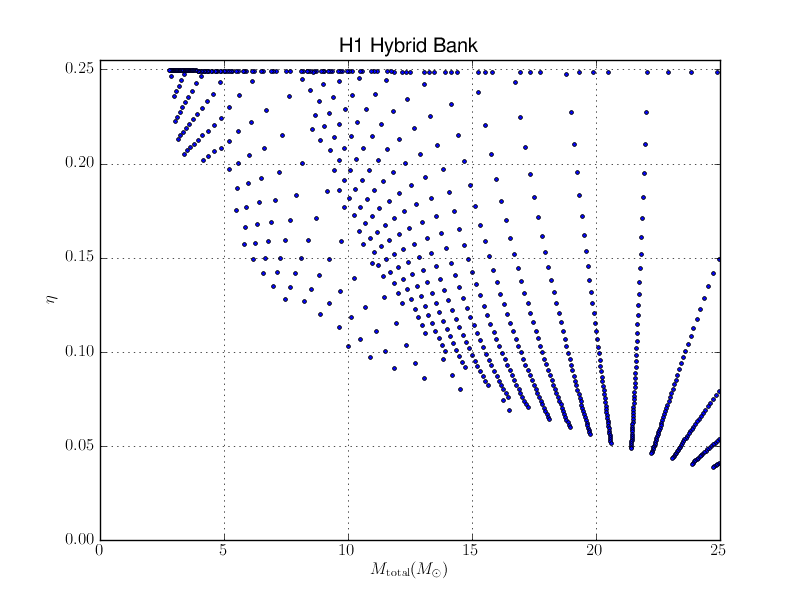
\includegraphics[width=\linewidth]{figures/detchar/hybrid_bank.png}
  \caption[The hybrid template bank used by daily ihope]{
  \label{f:daily_ihope_bank}
The hybrid template bank used by daily ihope for the Hanford detector,
the banks for L1 and V1 are similar.
The cut is made at constant chirp mass, which is
a curve in the total mass, $\eta$ plane.}
\end{figure}%

Daily ihope processing ran at 03:00 GMT and examined data spanning the
24 hours ending at 00:00 GMT.  Unlike full ihope, the analysis was
done on all science time, including that which would be vetoed at CAT
1 by the full analysis.  This was done so that we could see the effect
of the CAT 1 vetoes.  It is plausible, for example, that some such
vetoes would be too aggressive and we could decide based on the daily
results to include such times back into the analysis.  For consistency
science time was denoted CAT 0.  In addition CAT 3 vetoes to remove
hardware injections were not applied, so that we could see how many
injections would be lost by CAT 4 vetoes.  The daily pages therefore
displayed results for categories 0, 1, 2, and 4.

For each 2048-second chunk of contiguous data, at each IFO, the data
was run through each template in the bank and triggers selected as
described in section \ref{sec:analysis_trigger_selection}. For each
trigger $\chisq$ and new SNR were calculated and recorded.  Clustering
was then done in order to focus attention on glitches that were most
likely to cause problems in the full search.  Two sets of clustered
triggers were recorded using windows of 30 milliseconds and 16
seconds.  For each set the trigger with the largest value of new SNR
across all templates within the window length was recorded.

The triggers were also filtered.  A version of the veto definer file
designated as ``online'' was maintained and used by daily ihope to
identify times with veto categories.  These vetoed times were then
removed from the original and clustered files.  
% The pipeline is summarized in figure (xx).
The result is, for each 2048-second block in each ifo, 3 cluster
levels times 4 veto levels = 12 sets of triggers.

%do analysis
%record science triggers
%cluster 30 ms     determine cat 1
%cluster 16 sec    determine cat 1 + cat 2
%                  ...

%filter and record

\section{The Daily Ihope report pages}

Much of the utility of the daily runs was in the use of the resulting
triggers to identify data quality issues and quantify the value of
proposed vetoes.  Some of these uses will be discussed in
section~\ref{sec:applications}.  In addition to the triggers the daily
pipeline also produced a large number of plots and reports, organized
into web pages that were available to the collaboration.  Data
analysts could use these pages to spot potential problems for the full
analysis and begin more detailed followup studies.  

We now summarize the contents of the daily pages. Each report and plot
is made for each combination of the following:

\begin{itemize}
\item IFO: H1, L1 and V1
\item Cluster level: Unclustered, 30 ms clustering, 16 second
clustering
\item Veto level: Show all triggers in science time (level ``0''),
only those not removed by category 1 vetos, only those not
removed by categories 1 or 2, or only those note removed by
categories 1,2 and 4.  Hardware injections vetos (category 3) were not 
applied so that we could determine whether category 4 vetoes were 
remove them.
\end{itemize}

Each of these features could be set independently.  The top-level web
interface for a sample day is shown in figure~\ref{f:daily_ihope_top}.

\begin{figure}
  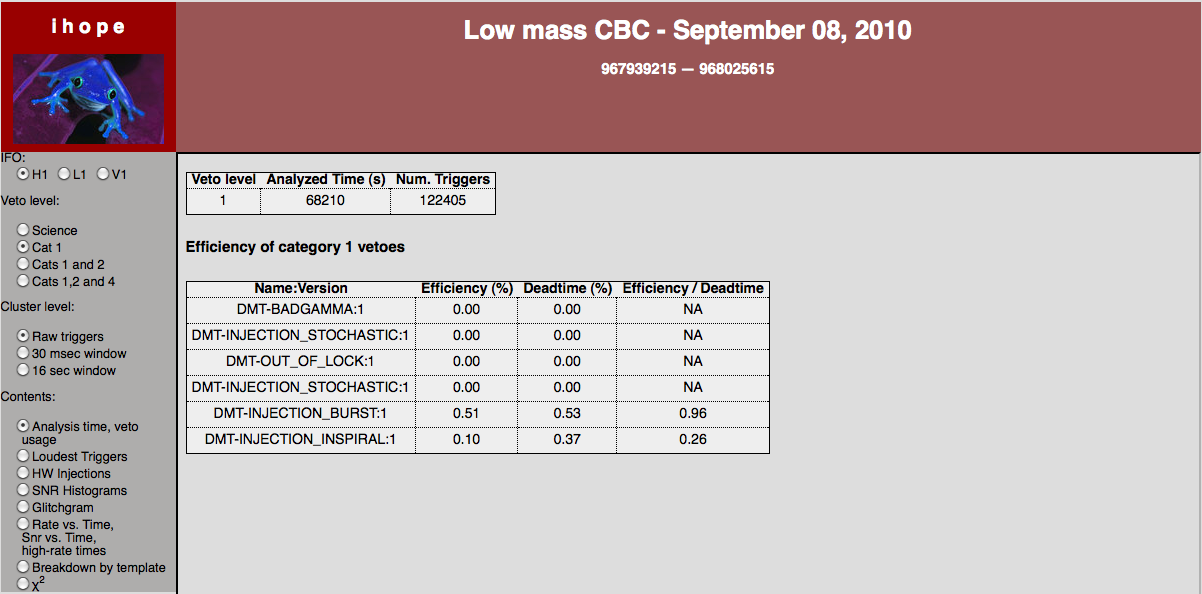
\includegraphics[width=\linewidth]{figures/detchar/daily_ihope_top}
  \caption[Top-level web interface for daily ihope]{
  \label{f:daily_ihope_top}
Top-level web interface for daily ihope.  Options can be selected with
the controls on the left hand side, when a button is clicked the
contents region is immediately replaced.  The default view is the one
shown here; the analysis time and veto efficiency at cat 1 for the
Hanford detector.}
\end{figure}%

The available reports can bee seen at the bottom of the list of
controls in figure~\ref{f:daily_ihope_top}:


1. Analysis time and veto usage.  This report shows the total time
analyzed, the vetoes applied beyond those applied at the previous
level, the \emph{efficiency} (percentage of triggers removed) and
\emph{deadtime} (percentage of time removed) by each veto.  In
addition the ratio of efficiency over deadtime is reported as a
measure of quality of the veto.  A random veto would result in an
efficiency-over-deadtime of approximately 1, a finely-tuned veto that
removes short, loud events that ring off the entire template bank
would have a much higher ratio.   An example is shown in
figure~\ref{f:daily_ihope_vetousage}.


\begin{figure}
  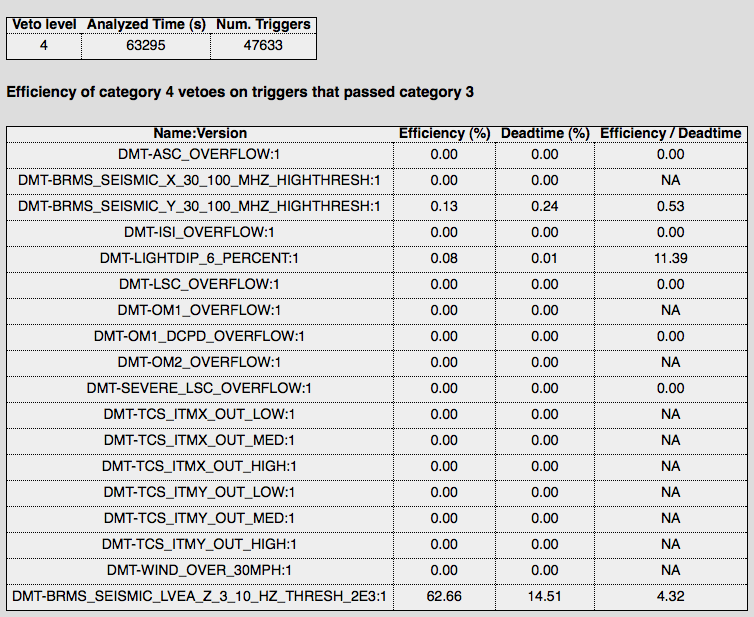
\includegraphics[width=\linewidth]{figures/detchar/vetousage.png}
  \caption[Sample veto usage report from Aug 19, 2010]{
  \label{f:daily_ihope_vetousage}
A sample veto usage report, see text for explanation.  Note that 62.66\% of
all triggers were contained in 14.51\% of time, and the DMT flagged this time
with elevated seismic activity from 3-10 Hz at the LVEA.}
\end{figure}%

2. Loudest triggers.  This report was only run for 16-second-clustered
triggers.  Loud glitches tend to produce families of triggers, without
clustering the loudest triggers from each day would likely result from
one underlying event.  This report considers two classes of triggers;
those where no data quality flag was active and those where at least
one flag was active.  A sample report is shown in
figure~\ref{f:daily_ihope_loudest}.  For the five triggers with
highest new SNR in each category a summary was presented along with a
link to an \emph{omega scan}.  The omega pipeline is described in
(\checkme{omega refs}).  Omega scans are a kind of time-frequency
plot.  They are especially useful as they may be run on all auxiliary
channels recorded by the instruments and therefore provide a visual
aid to detecting coupling between auxiliary channels and the
gravitational wave readout channel.  These can be used to suggest
mechanisms behind glitches, especially those that were not already
marked by a DQ flag.  In addition, over time repeated shapes in the
omega scan can pinpoint underlying problems in the instruments that
need to be addressed.  A few images from one of the glitches in
figure~\ref{f:daily_ihope_loudest} is shown in
figure~\ref{f:daily_ihope_loudest_omega}.

\begin{figure}
  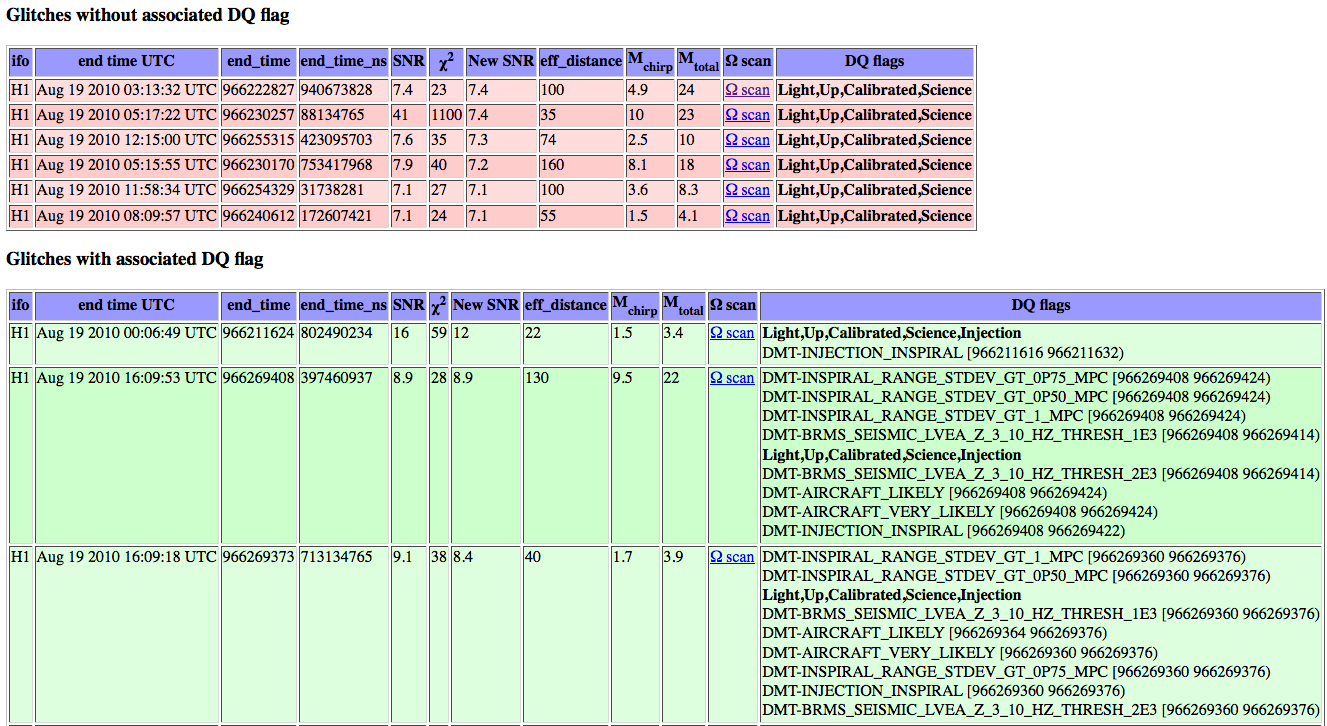
\includegraphics[width=\linewidth]{figures/detchar/loudest.png}
  \caption[Sample loudest trigger report from Aug 19, 2010]{
  \label{f:daily_ihope_loudest}
A sample report on loudest triggers, see text for explanation.  Note the
rightmost column is populated by
the \texttt{ligolw\_dq\_query} program in the \texttt{--report} mode.}
\end{figure}%



\begin{figure}
  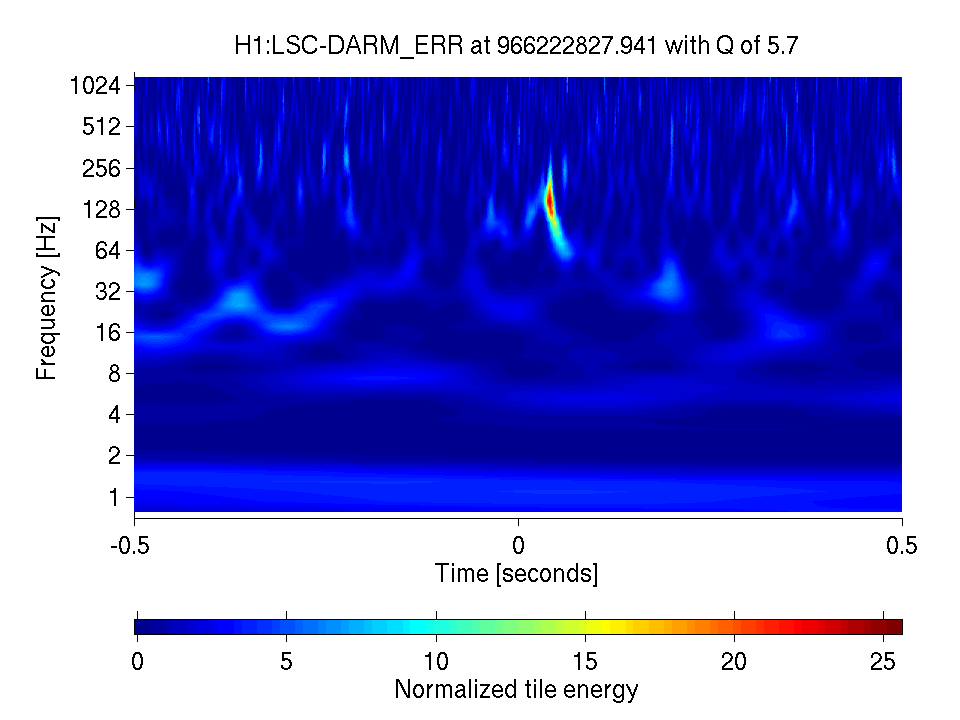
\includegraphics[width=0.5\linewidth]{figures/detchar/966222827_940673828_H1_LSC-DARM_ERR_1_00_spectrogram_whitened.png}
  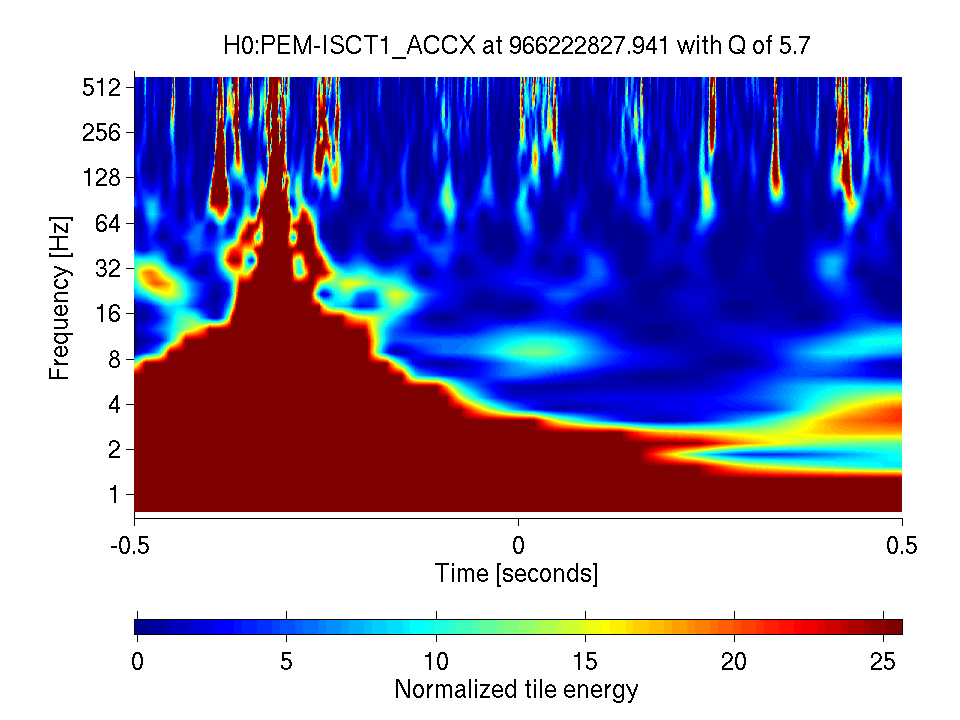
\includegraphics[width=0.5\linewidth]{figures/detchar/966222827_940673828_H0_PEM-ISCT1_ACCX_1_00_spectrogram_whitened.png}
  \caption[Omega scans from the loudest H1 trigger in figure \ref{f:daily_ihope_loudest}]{
  \label{f:daily_ihope_loudest_omega}
Omega scans from the loudest H1 trigger in figure
\ref{f:daily_ihope_loudest}.
Note the trigger closely follows a loud
event in one of the accelerometers on an instrument table.}
\end{figure}%


3. Hardware injections.  This report was generated by code written by
John Veitch  at Cardiff University.  It compared the list of
injections, published as an XML file available from a web site, with
the list of analysis times and triggers.  The results were plotted to
indicate whether each injection was found, missed, or not analyzed.



4. Hardware injections.  These plots show the number of triggers as a
function of SNR and new SNR.  As noted in section
\ref{sec:ihope_match_filter}, in Gaussian noise the number of triggers
should be proportional to $\exp(-\rho^2/2)$.  These plots therefore
show the degree of ``non-Gausianity'' in the data.  A common use for
these plots was to flip between veto levels to get a sense of how well
the cumulative vetoes were cleaning the data, as shown in figure
\ref{f:daily_ihope_gaussianity}.

Similarly figure~\ref{f:daily_ihope_new_hists} shows histograms of the
triggers in new SNR.  The total number of triggers is greatly reduced
because many high-SNR triggers have new SNR values below 5, where the
plot cuts off.  While triggers with such low new SNR values are not
excluded from later stages of analysis in the full pipeline, it is
extremely unlikely that the resulting combined new SNR will be high
enough to stand above background.

In addition the lower overall number of triggers, the new SNR plot is
closer to a straight line, indicating behavior closer to that expected
in Gaussian noise.  However, detchar improves the situation still
further, as the number of triggers is reduced at veto category 4.

However, there is one trigger with new SNR of 8 that is not removed by
any veto.  Such an outlier warrants further investigation, which here
is provided by the loudest events page described in
section~\ref{ihope_loudest}.  The omega scan from the time of this
event is shown in figure~\ref{f:daily_loudest_glitch}, and it clearly
rules out a gravitational wave as the source of this trigger.  This
illustrates the important point that new SNR can be fooled, and hence
continued human participation in detchar is necessary.

\begin{figure}
  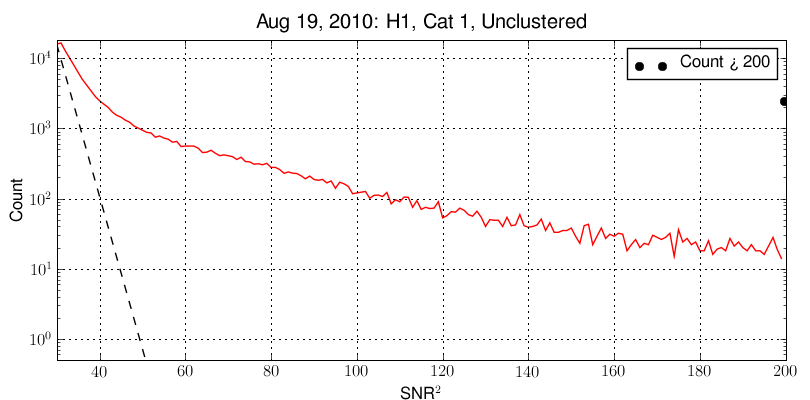
\includegraphics[width=0.5\linewidth]{figures/detchar/H1_1_UNCLUSTERED_snr_hist.png}
  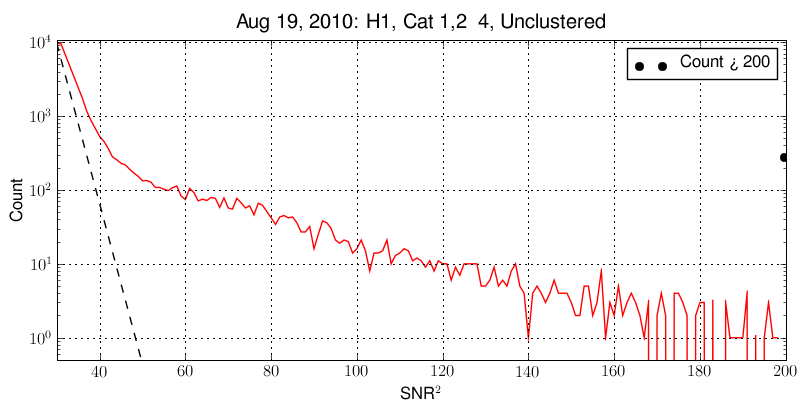
\includegraphics[width=0.5\linewidth]{figures/detchar/H1_4_UNCLUSTERED_snr_hist.png}
  \caption[Trigger SNR histograms for H1]{
  \label{f:daily_ihope_gaussianity}
Sample trigger histograms by SNR.  The dashed line shows the
expected values in Gaussian noise.  The dot indicates the cumulative
number of triggers with new SNR greater than 200.  Note that at veto
category 4 (right) the histogram is closer to the expected line than
it is at category 1 (left).  This indicates the degree to which data
quality has removed non-Guassian noise.}
\end{figure}%



\begin{figure}
  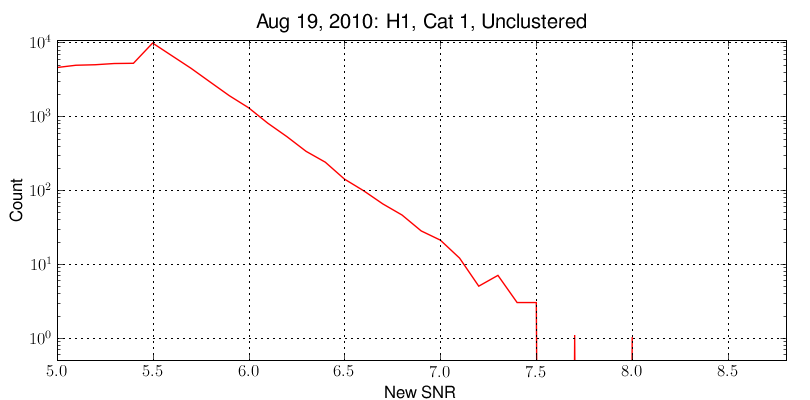
\includegraphics[width=0.5\linewidth]{figures/detchar/H1_1_UNCLUSTERED_new_snr_hist.png}
  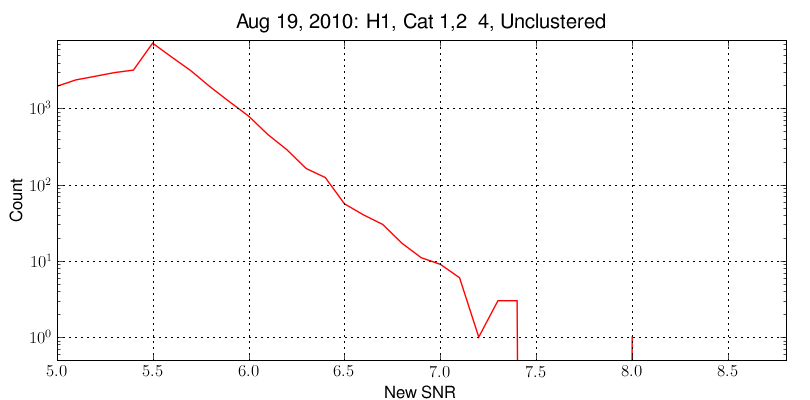
\includegraphics[width=0.5\linewidth]{figures/detchar/H1_4_UNCLUSTERED_new_snr_hist.png}
  \caption[Trigger new SNR histograms for H1]{
  \label{f:daily_ihope_gaussianity}
Sample trigger histograms by new SNR. The data is much cleaner than
the new SNR histograms, but there is still an outlier.}
\end{figure}%



\begin{figure}
  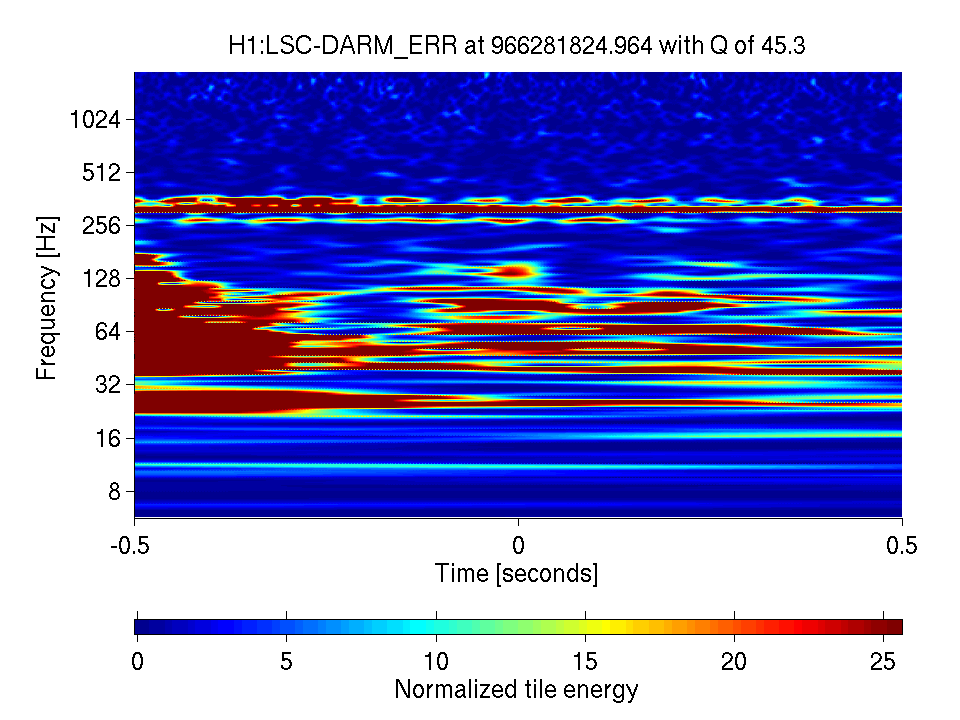
\includegraphics[width=\linewidth]{figures/detchar/966281824_963867187_H1_LSC-DARM_ERR_1_00_spectrogram_whitened}
  \caption[Omega scan of the loudest new SNR trigger]{
  \label{f:daily_loudest_glitch}
The omega scan from the outlier with new SNR=8 that survives all
automated data quality vetoes.  Many auxiliary channels showed the
same behavior at this time.  This is clearly not a gravitational wave,
but was not removed by either signal-based vetoes or data quality
vetoes.}
\end{figure}%



5. The ``glitchgram'' was an ``at-a-glance'' summary of the day,
showing every trigger color-coded by SNR.  This highlighted times of
loud triggers as well as dense regions indicating ``grumbly'' times.
A sample is shown in figure \ref{f:daily_ihope_glitchgram}.

\begin{figure}
  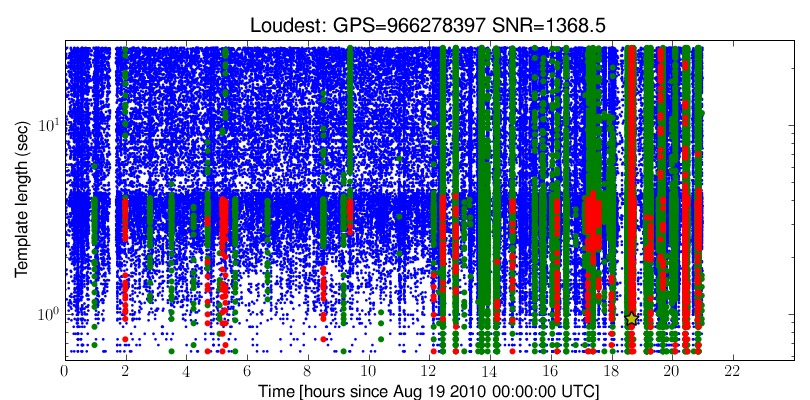
\includegraphics[width=\linewidth]{figures/detchar/H1_1_UNCLUSTERED_glitchgram.png}
  \caption[The Aug 19th daily ihope ``glitchgram'']{
  \label{f:daily_ihope_glitchgram}
A sample ``glitchgram.'' Blue dots have
new snr values below 8, green have values between 8 and 16,
and red have values above 16.  Template length was chosen as the Y
axis in order to capture a feature of the templates that is not
specific to gravitational wave signals, such as chirp mass.
Note the break at 4.3 seconds, corresponding to the
chirp mass at which the bank switches from an overlap of 0.95 to 0.5.
Comparing to figures 3 and 4 shows the same 
excess of triggers after 12:00.  No data is analyzed after 21:00
because ihope requires at least 2048 contiguous seconds to estimate
the PSD and all data after this time was in smaller segments.}
\end{figure}%


6. Rate vs. Time and SNR vs. Time.  These plots complimented the
glitchgram by breaking the triggers up differently.  The rate plot
(figure~\ref{f:daily_ihope_rate_v_time}) showed average number of
triggers over 1-minute intervals.  The SNR plot
(figure~\ref{f:daily_ihope_snr_v_time}) showed the SNR of every
trigger as a function of time.  These tend to be correlated, as loud
glitches ring off the entire bank and produce large numbers of
triggers.  The plots were accompanied by tables showing the times
where the rate of triggers exceeded 500 Hz for more than one second,
and exceeded 200 Hz for more than 10 seconds.

\begin{figure}
  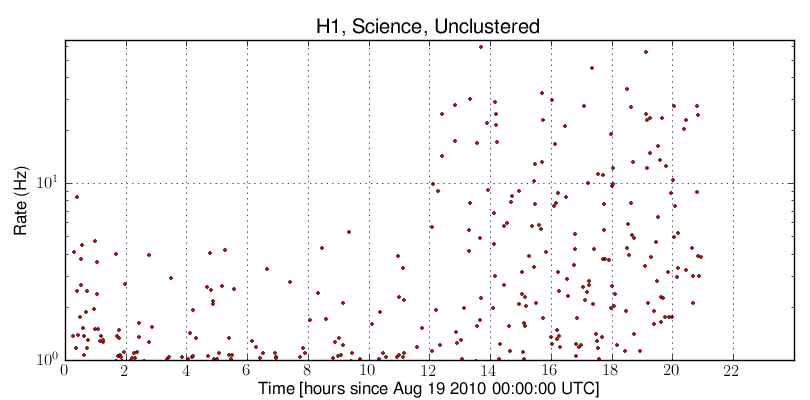
\includegraphics[width=\linewidth]{figures/detchar/H1_0_UNCLUSTERED_rate_vs_time.png}
  \caption[Daily ihope rate plot]{
  \label{f:daily_ihope_rate_v_time}
Sample rate plot, showing rate in Hz (averaged over
1-minute intervals) as a function of time.  Note that the rates
increase after 12:00.  This was due to increased seismic noise.}
\end{figure}%

\begin{figure}
  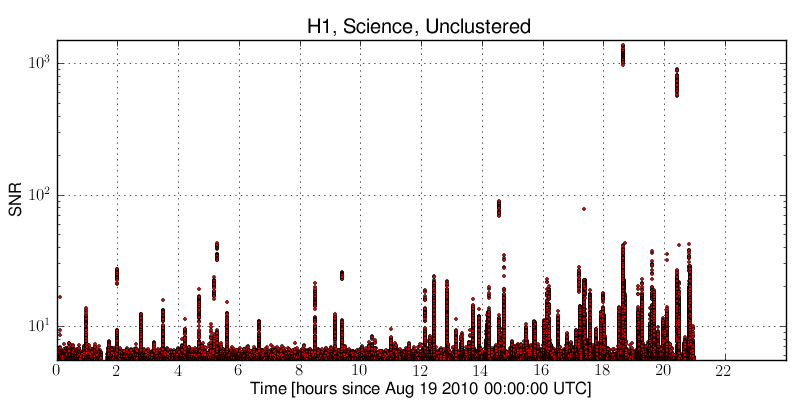
\includegraphics[width=\linewidth]{figures/detchar/H1_0_UNCLUSTERED_snr_vs_time.png}
  \caption[Daily ihope SNR plot as a function of time]{
  \label{f:daily_ihope_snr_v_time}
Sample plot of SNR as a function of time.  The density of
triggers increases somewhat after 12:00 and there are more loud
outliers.  However the change in behavior is better seen in 
figure \ref{f:daily_ihope_rate_v_time}.}
\end{figure}%


7. Breakdown by template.  This page showed several histograms of
number of triggers as a function of the length of templates in
seconds.  Examples of the standard histograms are shown in
figure~\ref{f:daily_ihope_trig_histograms}, they show that most of the
triggers come from short templates, and templates shorter than 5
seconds produce up to six times as many triggers as shorter templates.

Figure~\ref{f:count_per_template} shows the same information as a map
of the template bank, color-coded to indicate how many triggers each
template produced.  Figure~\ref{f:daily_ihope_time_mass} breaks this
same information up by time and template mass.

Qualitatively these plots do not change much day-by-day, and so these
plots were not often used.  However, they did prompt a change to
the analysis made early in the S6 run, see
section~\ref{sec:daily_pipeline_changes}.

\begin{figure}
  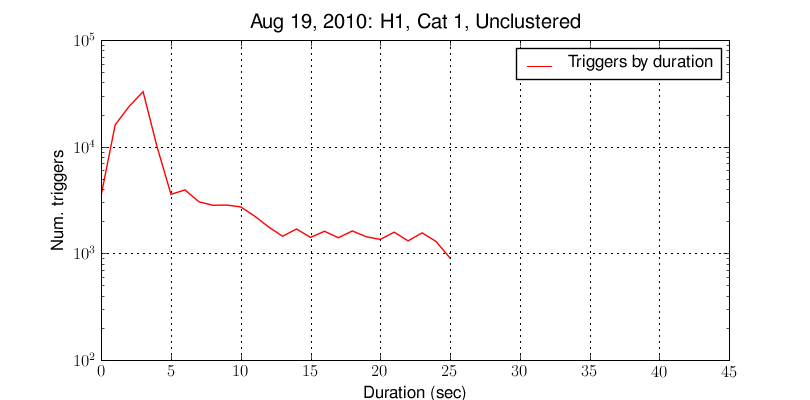
\includegraphics[width=0.5\linewidth]{figures/detchar/H1_1_UNCLUSTERED_mass_hist}
  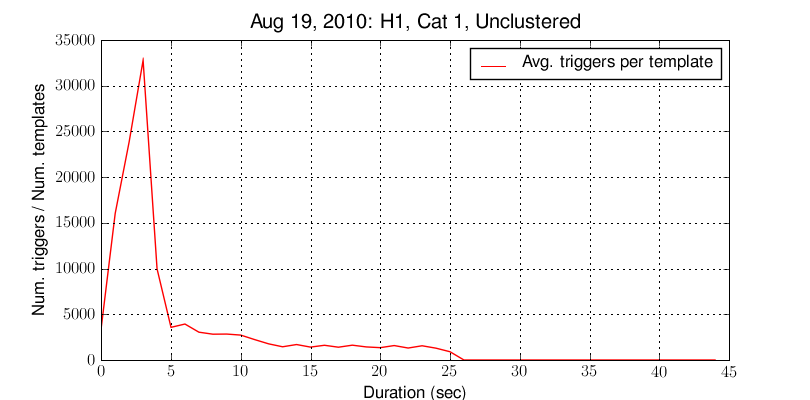
\includegraphics[width=0.5\linewidth]{figures/detchar/H1_1_UNCLUSTERED_mass_hist_norm}
  \caption[Histograms of trigger rates by template length]{
  \label{f:daily_ihope_trig_histograms}
Histograms of trigger rates by template length in daily ihope.  The
plot on the left combines all templates, the plot on the right
normalizes by plotting (number of triggers resulting from templates of
length $x$) divided by (number of templates of length $x$).
}
\end{figure}%

\begin{figure}
  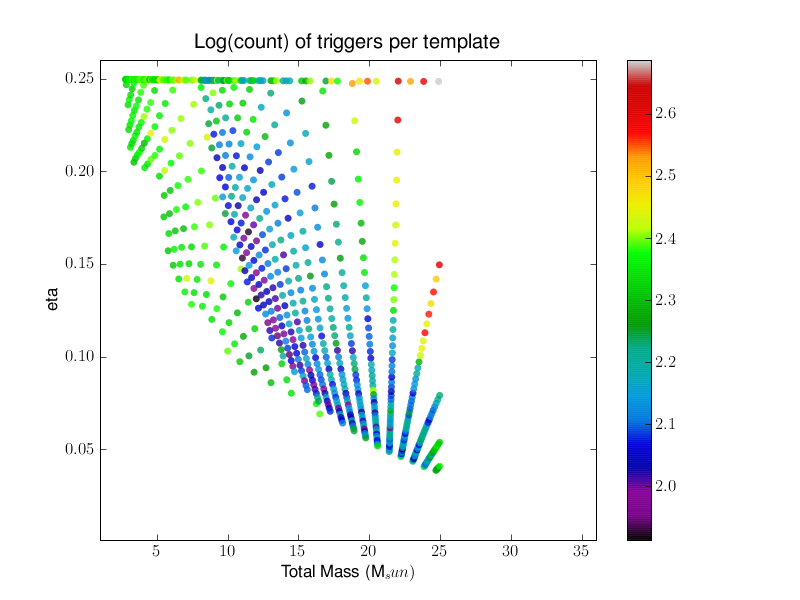
\includegraphics[width=\linewidth]{figures/detchar/H1_1_UNCLUSTERED_template_counts}
  \caption[Triggers per template]{
  \label{f:count_per_template}
The daily template bank, color-coded to show how many triggers each
template produced.  Note that the template in the upper-right corner,
which is the template of shortest duration, produced approximately 1.3
times as many triggers as the next most active.
}
\end{figure}%


\begin{figure}
  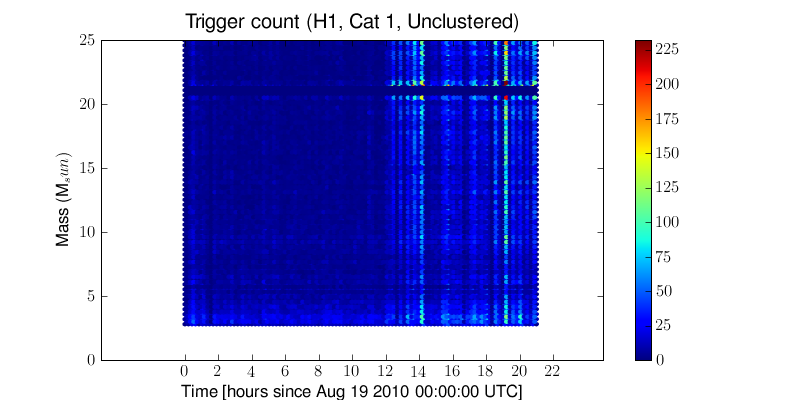
\includegraphics[width=\linewidth]{figures/detchar/H1_1_UNCLUSTERED_hexmass}
  \caption[Trigger rates as a function of time and template length]{
  \label{f:daily_ihope_time_mass}
Trigger rates as a function of time and template length.  The elevated
trigger rate after 12:00 is visible here as well.  Note that
particularly loud glitches, such as that around 19:30, ring off the
entire bank.
}
\end{figure}%


8.  The $\chisq$ test.  These plots showed all triggers in with SNR
values on the $x$-axis and $\chisq / (2p-2)$ (the reduced $\chisq$) on
the $y$-axis as a way to visualize the glitchiness of the data.  These
plots are most useful when compared to a reference plot generated from
a day of simulated Gaussian noise, shown in figure
\ref{f:gaussian_snr_chisq}, and comparing the plots at different veto
levels, shown in figure \ref{f:daily_ihope_snr_chisq}.

\begin{figure}
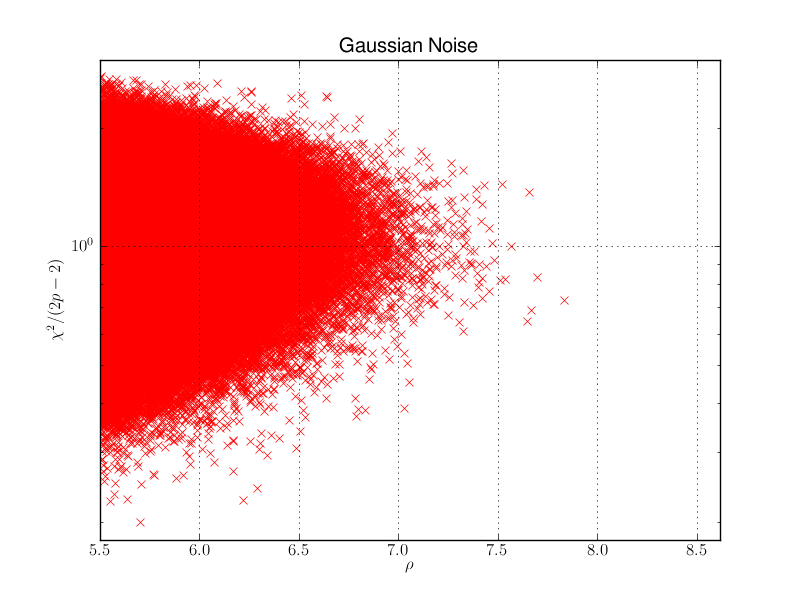
\includegraphics[width=0.85\linewidth]{figures/detchar/GAUSSIAN_0_UNCLUSTERED_chisq.png}
\caption[SNR/reduced $\chisq$ values in Gaussian noise]{
\label{f:gaussian_snr_chisq}
The SNR/reduced $\chisq$ plane for a reference day of
Gaussian noise.  This is the product of a $\chisq$ distribution on the
$y$ axis and a Gaussian distribution on the $x$ axis.}
\end{figure}%

\begin{figure}
  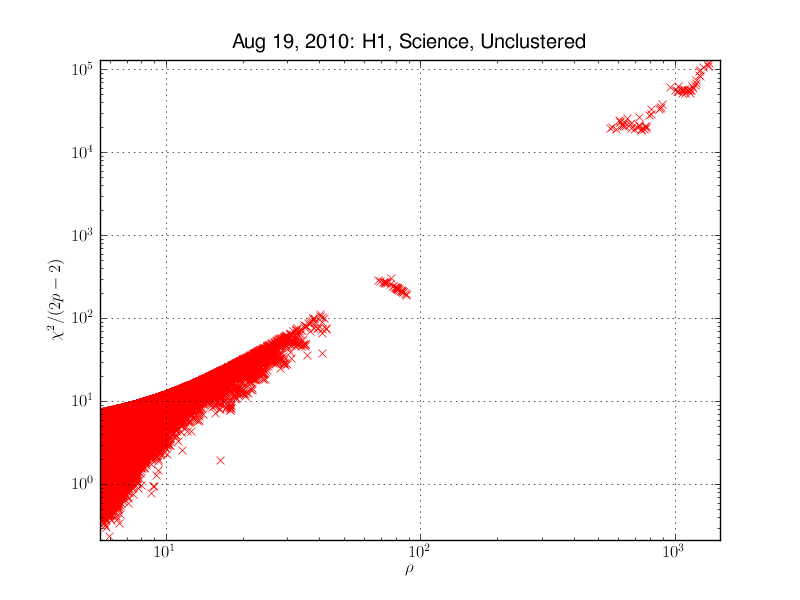
\includegraphics[width=0.5\linewidth]{figures/detchar/H1_0_UNCLUSTERED_chisq.png}
  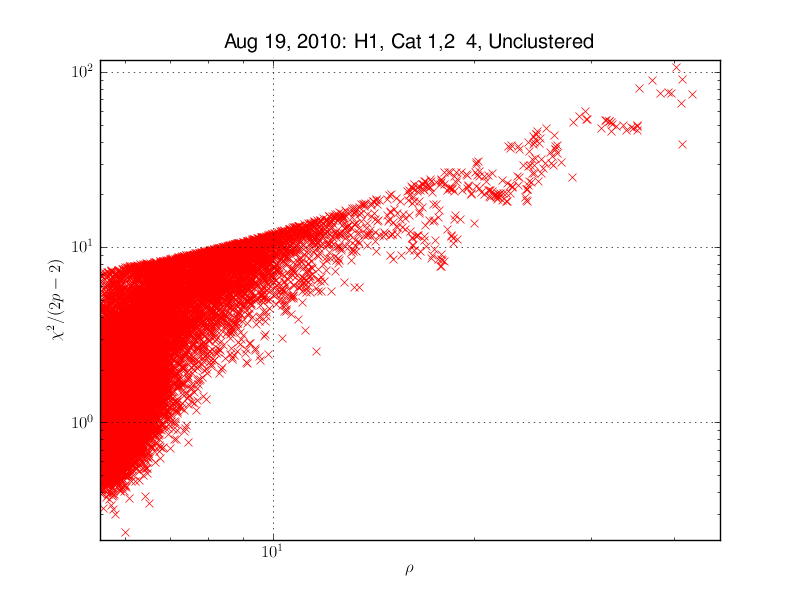
\includegraphics[width=0.5\linewidth]{figures/detchar/H1_4_UNCLUSTERED_chisq.png}
  \caption[SNR/reduced $\chisq$ plots of H1 data.]{
  \label{f:daily_ihope_snr_chisq}
SNR/reduced $\chisq$ plots of H1 data.  The expected shape
of figure \ref{f:gaussian_snr_chisq} is discernible, but there are
long tails of non-Gaussian glitches.  The sharp cutoffs arise 
from thresholds within the inspiral code, see section
\ref{sec:analysis_trigger_selection}.  There is a further
population extending to the upper right at category 0 (left) that is
removed by vetoes in category 4 (right).}
\end{figure}%


\section{Applications of daily ihope to pipeline tuning}

Early in S6 there were frequent instances where the full analysis ran
into difficulty.  This was characterized by individual programs taking
abnormally long to complete, consuming far more than the expected
amount of memory, or failing outright.  The problematic jobs tended to
be {\texttt trigbank} instances; this is the step where triggers from
the first stage are examined to determine which templates need to be
used at the second stage (see figure~\ref{f:hipe}).  Comparing the
times that caused problems to the daily pages immediately revealed a
correlation -- times over which trigscan were unable to run were those
where the rates of triggers were abnormally high.

In S5 and the early weeks of S6 triggers were clustered using a method
called {\emph trigscan}~\cite{SenguptaTrigScan:2008} which attempts to
collapse clusters of triggers that are close in time and parameters to
a single most-significant trigger.  Early versions of the daily page
did this clustering as well, and comparison between the unclustered
and trigscan-clustered triggers revealed that even after clustering
periods of high trigger rates remained~\footnote{Trigscan worked well
in S5, it is not known why it did not work as well in S6.  It is
possible that the instruments were simply more glitchy in the early
days of S6.  However, in order to group triggers together trigscan
must use the bank metric, which was correct in S5 when 2.0 pN
templates were used but incorrect in S6 when the analysis moved to 3.5
pN templates (see section~\ref{sec:bank_metric}).  Some preliminary
investigations were performed, but results were inconclusive}.  This
is illustrated in figure~\ref{f:daily_ihope_high_rates}.  There is a
short period of high trigger rate around 05:40 which remained high
after clustering.  A {\texttt trigbank} instance processing this time was
unable to complete.

The possibility of vetoing such glitchy periods was raised, and it
would have been easy to accomplish using the rate information from
daily ihope.  However, such vetoes would have needed to be category 1 to
avoid the problem, which would mean subdividing science segments and
possibly losing short segments.  Instead we replaced trigscan with
fixed 30-millisecond clustering windows, after studies of found/missed
injections determined that this change did not harm the search
efficiency. 

\begin{figure}
  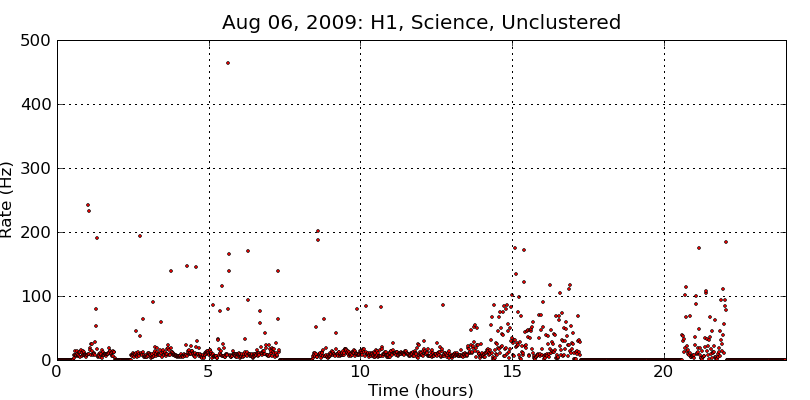
\includegraphics[width=0.5\linewidth]{figures/detchar/20090806_H1_0_UNCLUSTERED_rate_vs_time}
  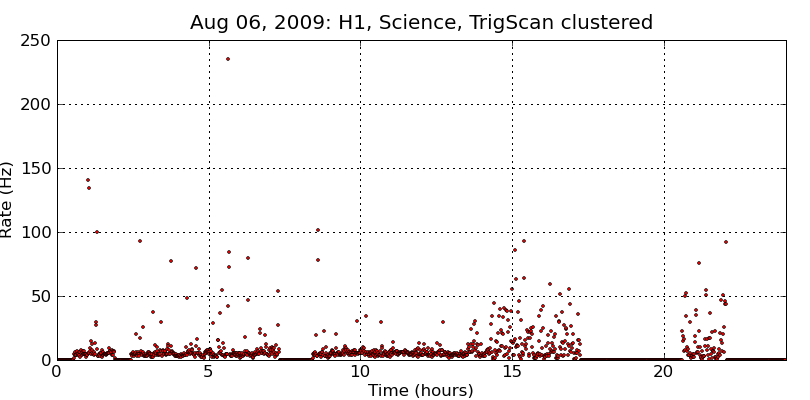
\includegraphics[width=0.5\linewidth]{figures/detchar/20090806_H1_0_TS_CLUSTERED_rate_vs_time}
  \caption[Problematic times identified by daily ihope]{
  \label{f:daily_ihope_high_rates}
}
\end{figure}%

At the start of S6 the range of the low-mass search extended up to $35
\msun$, as it did in S5.  However, along with times of high trigger
rates, the daily ihope pages indicated that most of the triggers were
coming from the high-mass end of the bank.  This behavior is expected,
as it is easier for short templates to match against glitches, but the
trigger histograms highlighted the extent to which this was a problem.
A sample plot of triggers per template from early S6 is shown on the
left of figure~\ref{f:el_glitcho}.  It shows that the shortest
template in the bank, with $m_1 = m_2 = 17.5 \msun$ was producing
significantly more triggers than any other template.  In part this was
due to a bug in the template bank code, that caused this template to
appear twice in some banks.  In part the abundance of triggers from
this template is due to it appearing in every bank throughout the day,
whereas other templates tend to get repositioned as the noise curve
changes.  Even taking these effects into account, most of the triggers
come from templates shorter than \Note{value}, as seen on the right of
figure~\ref{f:el_glitcho}.  

The fixed clustering window means that only the loudest trigger in a
30-millisecond window will be passed to subsequent stages of the
analysis.  Given the numbers of triggers from short templates there
was concern that a loud, short glitch could mask a quieter trigger
from a binary neutron star coalescence.  We therefore decided to limit
the low-mass search to $M < 25 \msun$ \Note{mention studies done to
vet this decision}.




\begin{figure}
  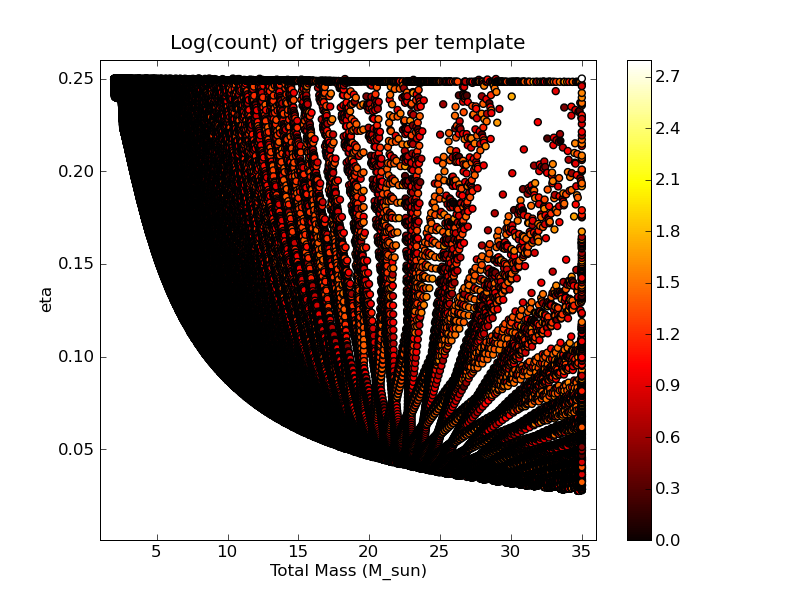
\includegraphics[width=0.5\linewidth]{figures/detchar/20090806_H1_0_UNCLUSTERED_template_counts}
  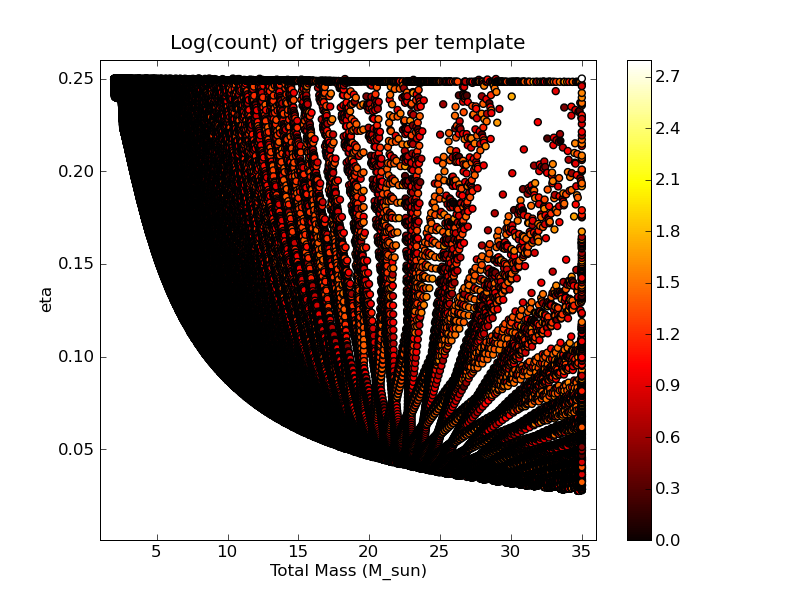
\includegraphics[width=0.5\linewidth]{figures/detchar/20090806_H1_0_UNCLUSTERED_template_counts}
  \caption[Problematic templates seen in daily ihope]{
  \label{f:daily_ihope_el_glitcho}
Problematic templates seen in daily ihope.  On the left the version 
of figure~\ref{f:count_per_template} from an earlier version of daily
ihope and an earlier version of the CBC search.  Note the excess of
triggers from the high-mass end of the bank.  On the right, a
histogram of trigger rates by template length more clearly indicating
that the high-mass is producing triggers at rates that could mask 
signals from lower-mass systems.
}
\end{figure}%



\section{Applications of daily ihope to individual vetoes}


\subsection{Category 1}

TCS

\begin{figure}
  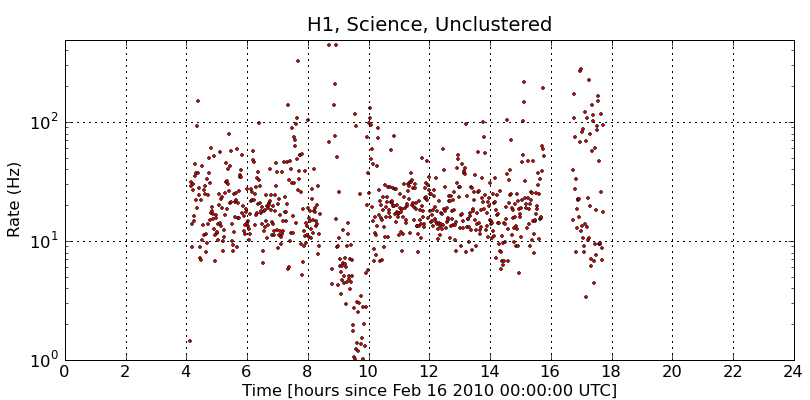
\includegraphics[width=0.5\linewidth]{figures/detchar/20100217_H1_0_UNCLUSTERED_rate_vs_time}
  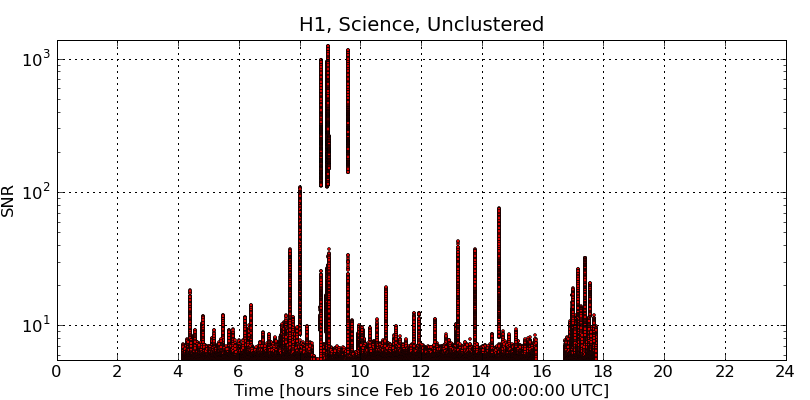
\includegraphics[width=0.5\linewidth]{figures/detchar/20100217_H1_0_UNCLUSTERED_snr_vs_time}
  \caption[TCS glitch in daily ihope]{
  \label{f:daily_ihope_snr_chisq}
}
\end{figure}%


\begin{figure}
  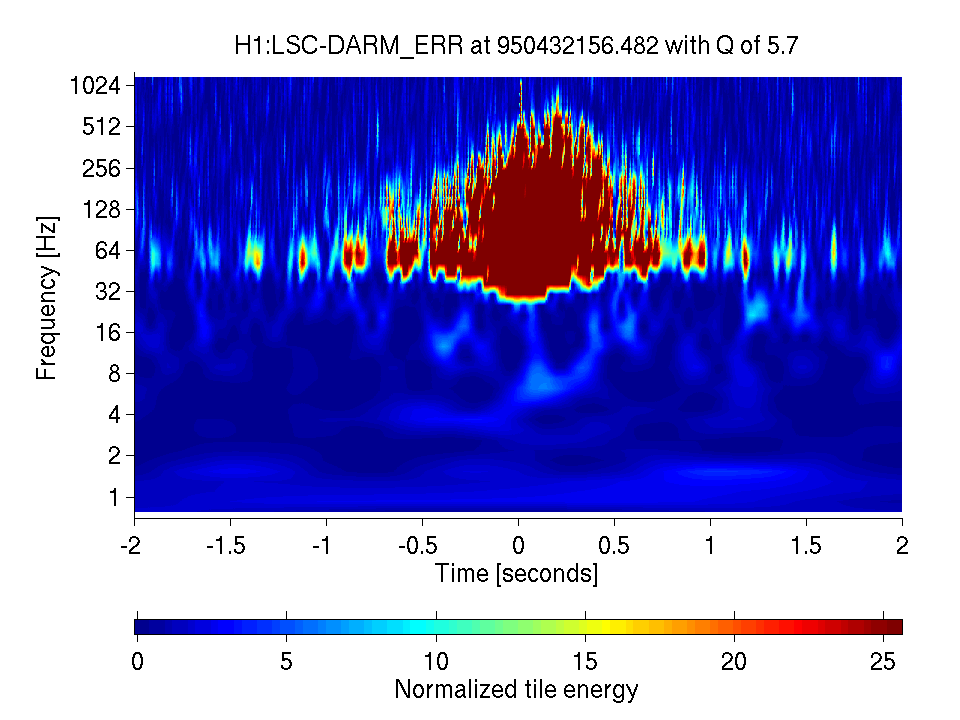
\includegraphics[width=0.5\linewidth]{figures/detchar/950432156_482177734_H1_LSC-DARM_ERR_4_00_spectrogram_whitened}
  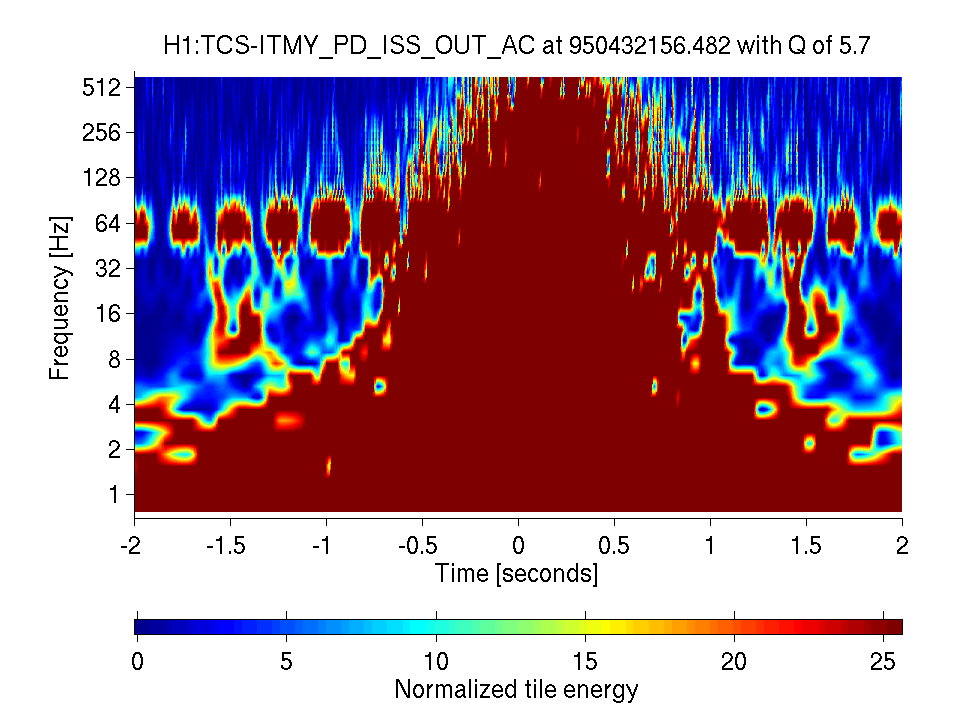
\includegraphics[width=0.5\linewidth]{figures/detchar/950432156_482177734_H1_TCS-ITMY_PD_ISS_OUT_AC_4_00_spectrogram_whitened}
  \caption[TCS glitch in omega]{
  \label{f:daily_ihope_snr_chisq}
}
\end{figure}%


Grid glitches

% https://wiki.ligo.org/foswiki/bin/view/DetChar/CurrentUnvetoedGlitchClasses
% https://wiki.ligo.org/DetChar/H1GridGlitchStory

% Example: 
% tconvert 963852915
% Jul 22 2010 16:55:00 UTC

\begin{figure}
  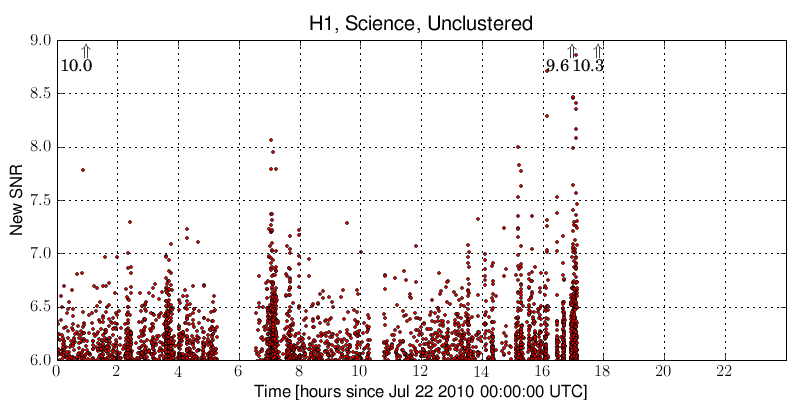
\includegraphics[width=0.5\linewidth]{figures/detchar/20100722_H1_0_UNCLUSTERED_newsnr_vs_time}
  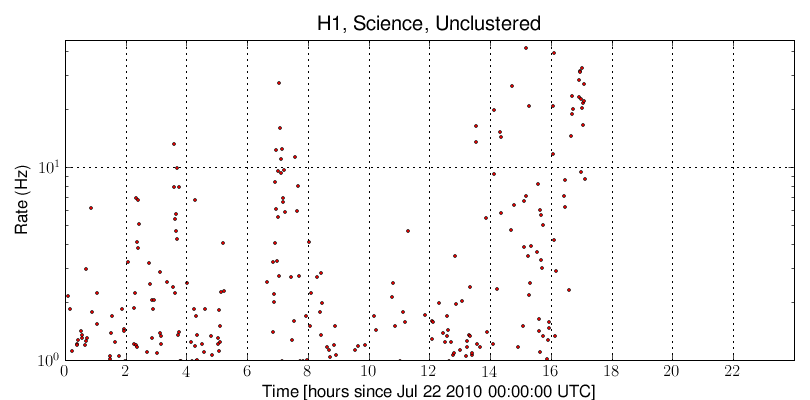
\includegraphics[width=0.5\linewidth]{figures/detchar/20100722_H1_0_UNCLUSTERED_rate_vs_time}
  \caption[Grid glitches in daily ihope] {
}
\end{figure}%

\begin{figure}
  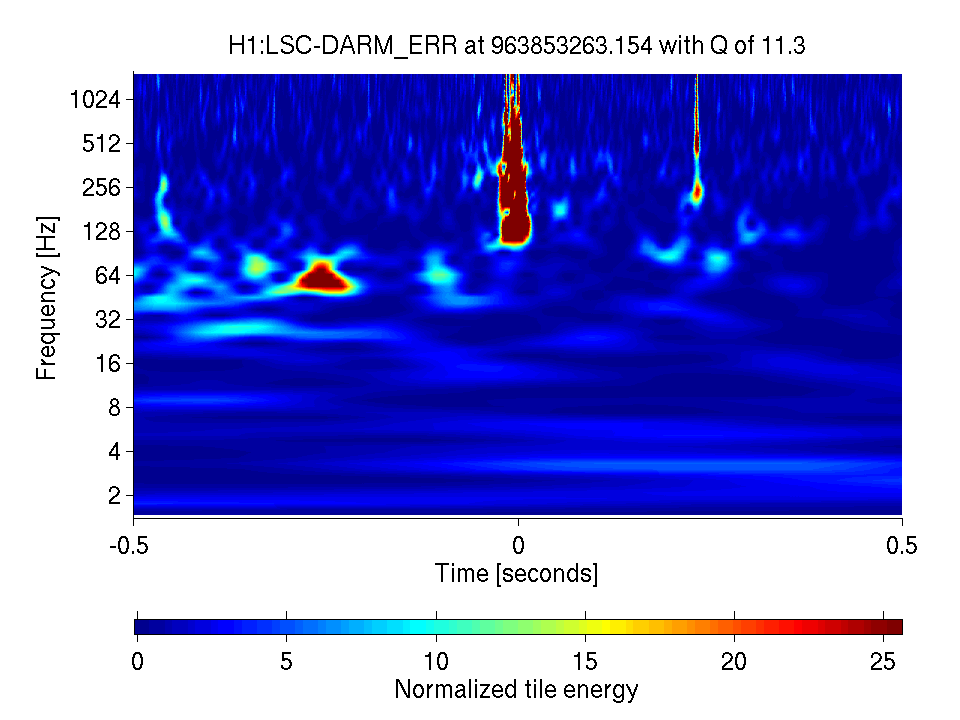
\includegraphics[width=\linewidth]{figures/detchar/963853263_154296875_H1_LSC-DARM_ERR_1_00_spectrogram_whitened}
  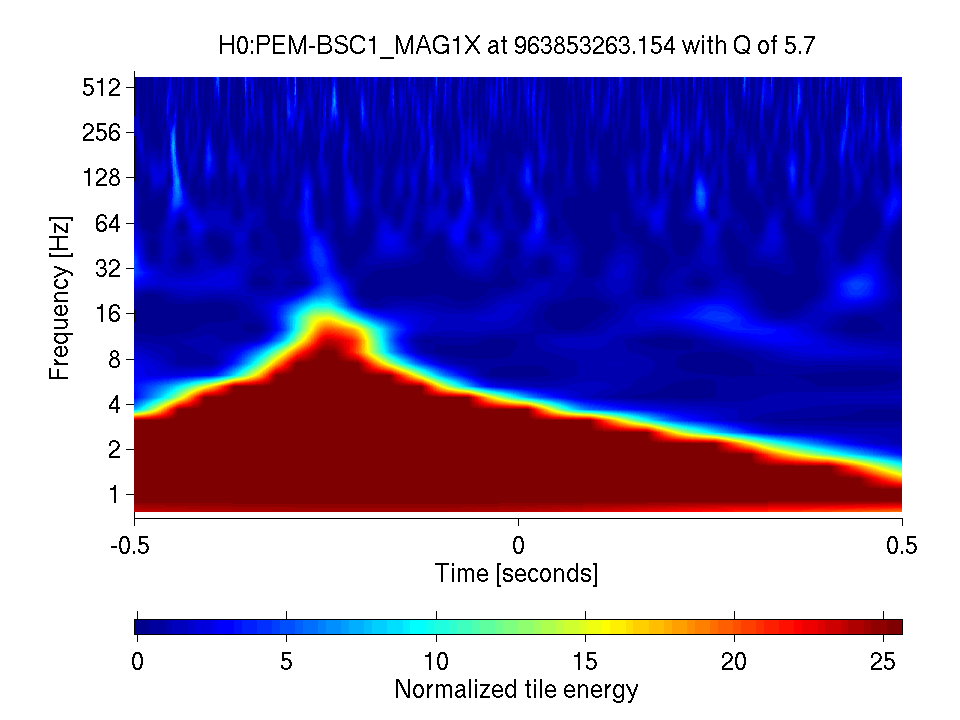
\includegraphics[width=0.5\linewidth]{figures/detchar/963853263_154296875_H0_PEM-BSC1_MAG1X_1_00_spectrogram_whitened}
  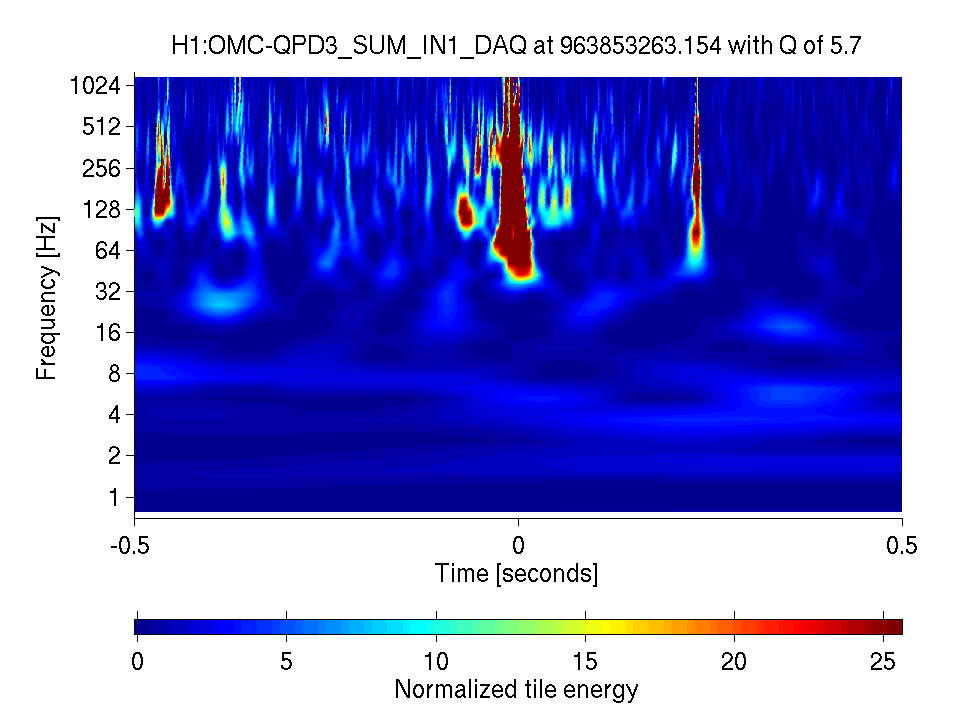
\includegraphics[width=0.5\linewidth]{figures/detchar/963853263_154296875_H1_OMC-QPD3_SUM_IN1_DAQ_1_00_spectrogram_whitened}
  \caption[Grid glitches in omega]{
}
\end{figure}%




\subsection{Category 2}

Spikes
% https://wiki.ligo.org/foswiki/bin/view/DetChar/S6L1OMCGlitchVeto

% DCH-SPIKE_GLITCH (0,4)

% Example 947204646.611816406
% Jan 11 2010 00:23:51.611816406 UTC == SNR 8849

\begin{figure}
  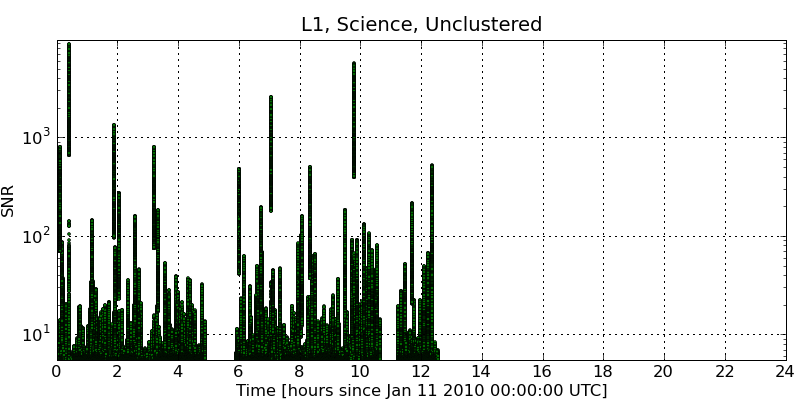
\includegraphics[width=\linewidth]{figures/detchar/20100111_L1_0_UNCLUSTERED_snr_vs_time}
  \caption[A spike glitch in daily ihope]{
}
\end{figure}

\begin{figure}
  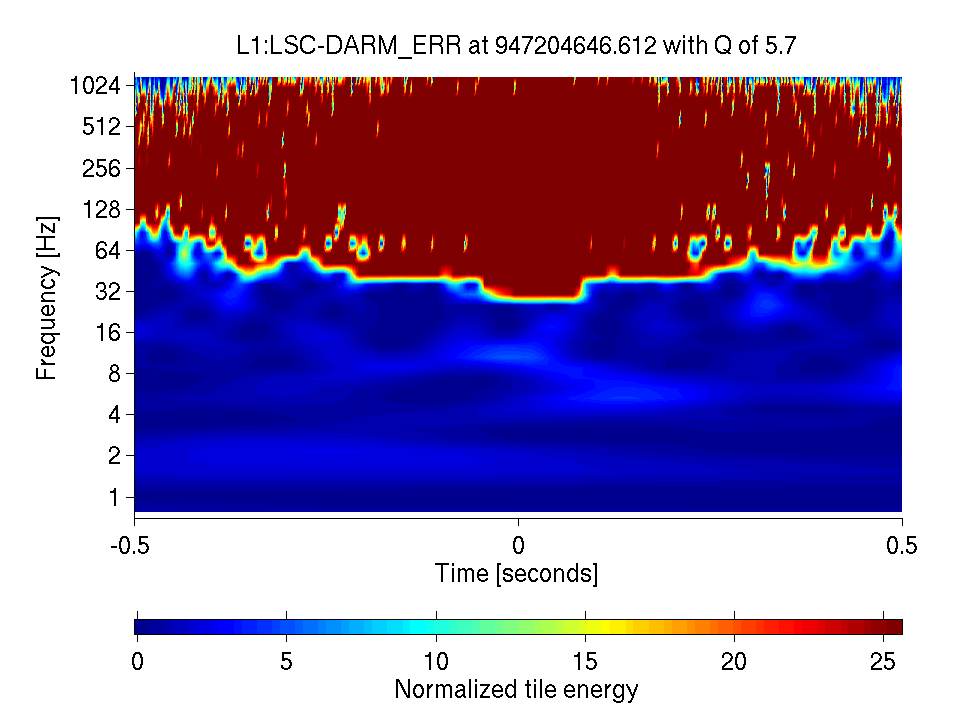
\includegraphics[width=0.5\linewidth]{figures/detchar/947204646_611816406_L1_LSC-DARM_ERR_1_00_spectrogram_whitened}
  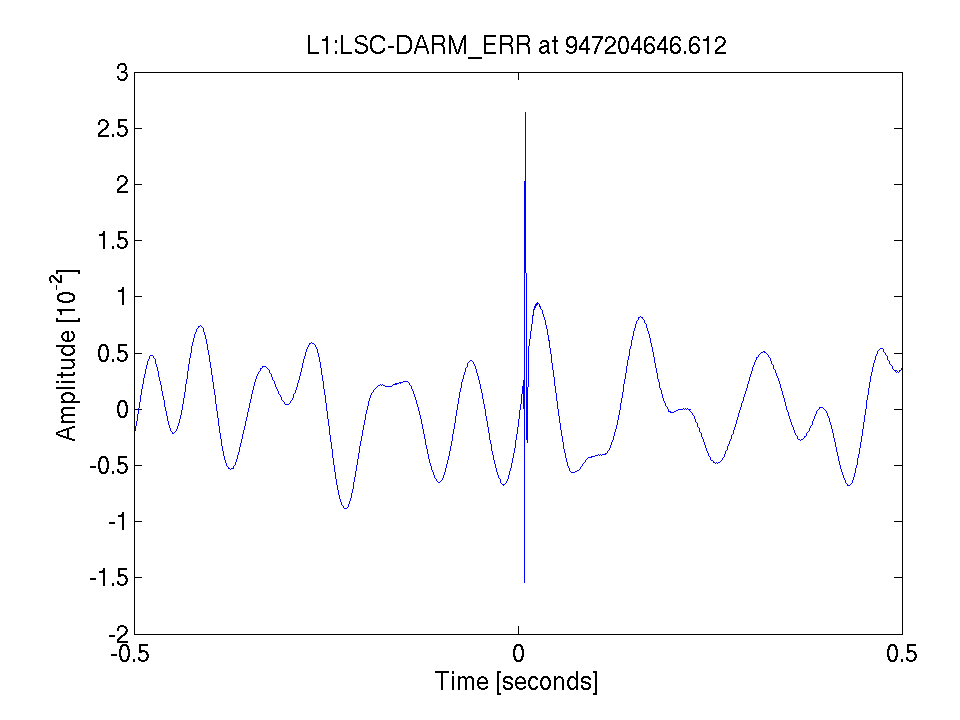
\includegraphics[width=0.5\linewidth]{figures/detchar/947204646_611816406_L1_LSC-DARM_ERR_1_00_timeseries_raw}
  \caption{Spike glitch in omega}
\end{figure}



Slips

% "L1","DCH-OMCLSC_SLIP",3,2,937473702,952387219,0,4,"Slip in OMC-LSC communications generated by hand until 952387215."
% Example 952339113.947204646
% Mar 11 2010 10:38:18 UTC == SNR 24
% Second loudest unflagged 
% on https://ldas-jobs.ligo.caltech.edu/~cbc/ihope_daily/201003/20100311/
% Doesn't really stand out in snr time series... there are too many
% loud flagged ones!


\begin{figure}
  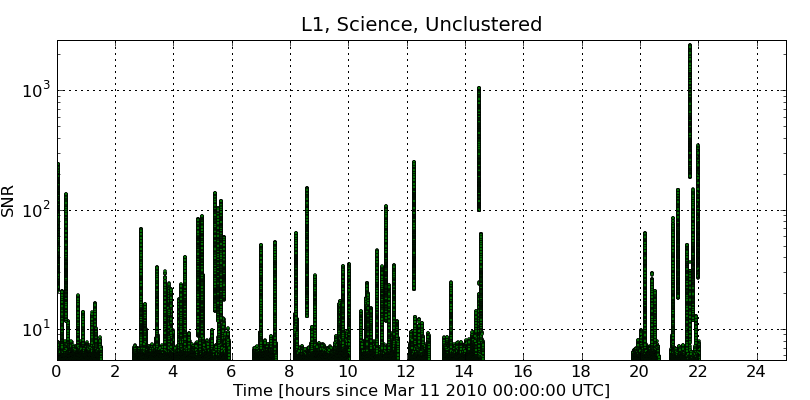
\includegraphics[width=\linewidth]{figures/detchar/20100311_L1_0_UNCLUSTERED_snr_vs_time}
  \caption[A slip glitch in daily ihope]{
}
\end{figure}

\begin{figure}
  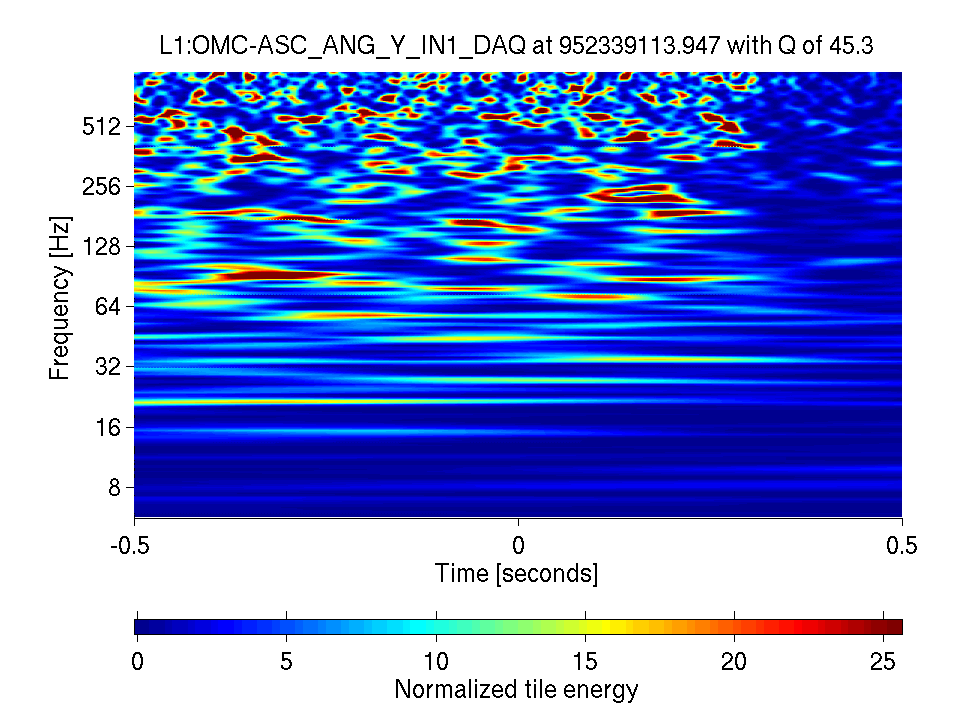
\includegraphics[width=0.5\linewidth]{figures/detchar/952339113_947204646_L1_OMC-ASC_ANG_Y_IN1_DAQ_1_00_spectrogram_whitened}
  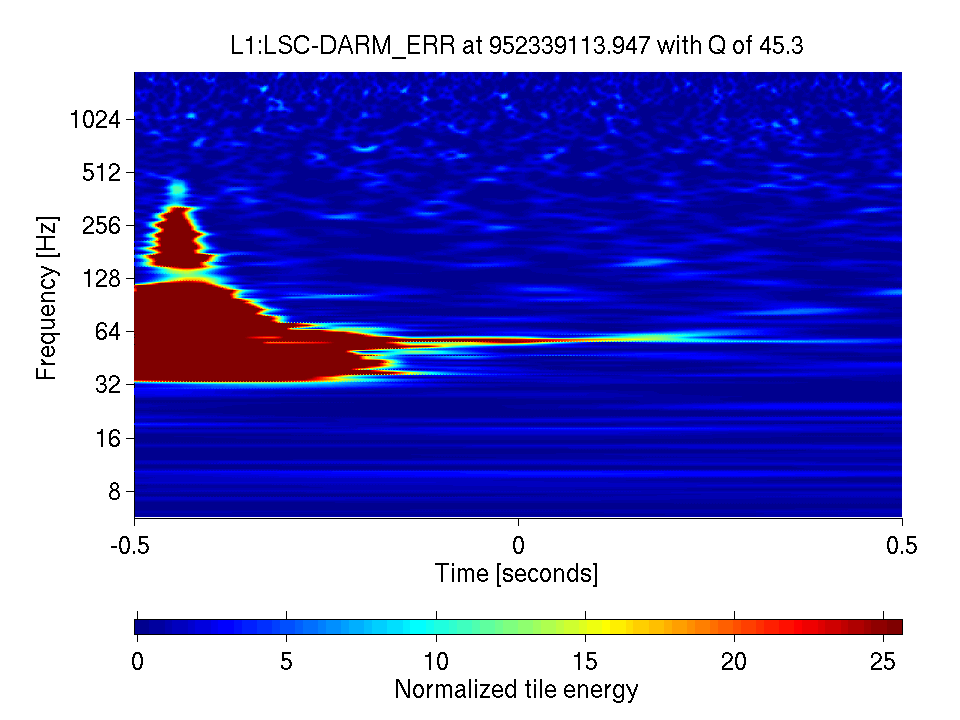
\includegraphics[width=0.5\linewidth]{figures/detchar/952339113_947204646_L1_LSC-DARM_ERR_1_00_spectrogram_whitened}
  \caption[Slip glitch in omega]{
}
\end{figure}




\subsection{Category 4}

% https://wiki.ligo.org/foswiki/bin/view/DetChar/H1LVEASEISZS6Cflag

\iffalse

UPV-IHOPE_H1_ASC_WFS2_IY_8_256_100 (in C) and more

Eg (tconvert 957092703, May 05 2010 11:04:48 UTC)

(tconvert 957191412, May 06 2010 14:29:57 UTC)
Accompanied by rate > 500 Hz for 4 seconds, slight elevation in SNR

DCH-SEISVETO_CBC
\fi

Loud SNR:

Through the S6 run the \emph{horizon distance}, the distance at which
the coalescence of an optimally-oriented binary system consisting of
two $1.4 \msun$ neutron stars would have an SNR of 8, was roughly 30
Mpc.  The SNR scales inversely with distance, hence the distance at
which we would expect to see such a system at, say, SNR 250 is 0.12
Mpc.  Assuming uniform volume distribution, this makes an SNR 250
event $6.4 \times 10^{-8}$ times less likely than an SNR 8 event.  
However, such loud glitches do occur in the data fairly often,
especially at L1 due to a glitch mechanism with a characteristic shape
but unknown cause.

Such loud glitches tend to have high $\chisq$ values which suppress
them.  However, around SNR 250 glitches tend to be accompanied by
additional triggers spanning $\pm 8$ seconds resulting from the
interaction of the filter with the inverse spectrum truncation, see
section \ref{sec:ihope_data_conditioning}.  Some of these auxiliary
triggers can, by chance, have low $\chisq$ values and hence high new
SNR values, and can potentially interfere with the search.  This
suggests a CAT 4 veto centered on times of triggers with SNRs
exceeding 250 with 8 seconds of padding in both directions.  Such a
flag must be in place before the full run, making daily ihope the
obvious choice for generating the flags.

This scheme was implemented starting on June 26, 2010, coinciding with
the portion of the run designated S6D.  An example of its
effectiveness is shown in table \ref{tab:daily_ihope_loud_flag} which
shows the efficiency and deadtime off the flag applied to triggers
from the full analysis after CAT 1, for the two weeks containing the
blind injection.  The efficiency to deadtime ratio is greater than 1,
although still relatively small.  Still, the flag was deemed useful as
it removed triggers we could not have easily claimed were due to a
gravitational wave.

\begin{table*}
\begin{center}
\begin{tabular}{lrrcrrcc}
\hline
ifo & Triggers & Vetoed & Efficiency & Time
& Vetoed & Dead-  & Ratio \\
 & (Count) & (Count) &  & (sec) & (sec) & time (sec) &  \\
\hline
L1  & 2890507 & 12578 & 0.43 & 798720 & 880 & 0.11 & 3.95 \\
H1  & 1692904 &  6452 & 0.38 & 647168 & 416 & 0.06 & 5.92 \\
\end{tabular}
  \caption[Effectiveness of the ``SNR $>$ 250'' flag]{
  \label{tab:daily_ihope_loud_flag}
Effectiveness of the ``SNR $>$ 250'' flag over the weeks
09/04/2010  to 09/17/2010.  Note that the flag was used almost twice
as often in L1 as H1, although there is only 23\% more analysis time.
This is another indication that L1 was glitchier overall.}
\end{center}
\end{table*}

\Note{Penguin discussion goes here}


\subsection{Non-vetoed time}

  https://www.lsc-group.phys.uwm.edu/ligovirgo/cbcnote/S6Vsr2Minutes20091027
    Andy: has started comparing S6a OMC slips against daily triggers,
    doesn't look like there's a problem. 

  https://www.lsc-group.phys.uwm.edu/ligovirgo/cbcnote/S6Plan/100216085311DQandVetoesS6B%20CAT1%20Flags
    Week 5,6: None of the circumstances noted in the scimon flags resulted in an excess or increased
    loudness of triggers. 

  https://www.lsc-group.phys.uwm.edu/ligovirgo/cbcnote/S6Vsr2Minutes20100614
    On week 17, use of daily to show something isn't a problem:
      Duncan B: Rates on the daily pages don't seem to be affected. Suggests
      that Ben does an investigation for next week, correlating the rate of
      daily ihope triggers with daily flow rates and site seismic. 



\section{Applications of daily ihope to the blind injection challenge}

In addition to the hardware injections discussed in section
\ref{sec:ihope_hardware_injections} it was known at the start of S6
that there would be any from zero to ``a few'' unannounced, blind
hardware injections performed in order to provide an unbiased test of
the search pipelines.  One such injection was performed on  Sep 16
2010 at 06:42 UTC, and showed up in multiple searches as a strong
gravitational wave candidate.  This candidate was followed up to the
point of writing a detection paper and submitting it to the
collaboration for publication approval.  Once approval had been
granted the fact that it had been an injection was revealed.  For more
details on the event and how it was followed up, see (the S6 low mass
paper).

Although daily ihope was not a search, the injection showed up on the
page of loudest triggers for H1 and L1, with parameters shown in table
\ref{tab:daily_ihope_dog} and omega scans shown in figure
\ref{f:daily_ihope_dog_omega}.  The injection was not visible in V1 in
daily ihope.


The daily ihope triggers were a useful resource in performing rapid
follow-up studies after the full ihope pipeline had been run and
identified the injection as a significant candidate.

\begin{landscape}
\begin{table*}
\begin{center}
\begin{tabular}{lllllllllll}
\hline
ifo & end\_time & end\_time\_ns & SNR & $\chisq$ & New SNR & Mchirp & DQ flags \\
\hline
H1  & 968654557 & 997314453 & 15 & 87 & 9.8 & 4.6 & DMT-INSPIRAL\_RANGE\_STDEV\_GT\_0P50\_MPC \\
    &           &           &    &     &    &     & \hspace*{0.5 in} [968654544 968654560) \\
    &           &           &    &     &    &     & DMT-INSPIRAL\_RANGE\_STDEV\_GT\_0P75\_MPC \\
    &           &           &    &     &    &     & \hspace*{0.5 in} [968654544 968654560) \\
    &           &           &    &     &    &     & Light,Up,Calibrated,Science \\
\hline
L1 & 968654557 & 978027343 & 9.9 & 44 & 8.7 & 4.1 & SCI-OTHER\_ELOG [967120215 977875215) \\
    &           &           &    &     &    &     & DMT-INSPIRAL\_RANGE\_STDEV\_GT\_1\_MPC \\
    &           &           &    &     &    &     & \hspace*{0.5 in} [968654544 968654560) \\
    &           &           &    &     &    &     & DMT-INSPIRAL\_RANGE\_STDEV\_GT\_0P50\_MPC \\
    &           &           &    &     &    &     & \hspace*{0.5 in} [968654544 968654560) \\
    &           &           &    &     &    &     & DMT-INSPIRAL\_RANGE\_STDEV\_GT\_0P75\_MPC \\
    &           &           &    &     &    &     & \hspace*{0.5 in} [968654544 968654560) \\
    &           &           &    &     &    &     & SCI-FLAG\_ERROR \\
    &           &           &    &     &    &     & \hspace*{0.5 in} [967137346 977875215) \\
    &           &           &    &     &    &     & Light,Up,Calibrated,Science \\
\hline
\end{tabular}
\end{center}
  \caption[Recovered blind injection parameters]{
  \label{tab:daily_ihope_dog}
The blind injection as reported by daily ihope's ``loudest triggers'' page.}
\end{table*}
\end{landscape}


\begin{figure}
  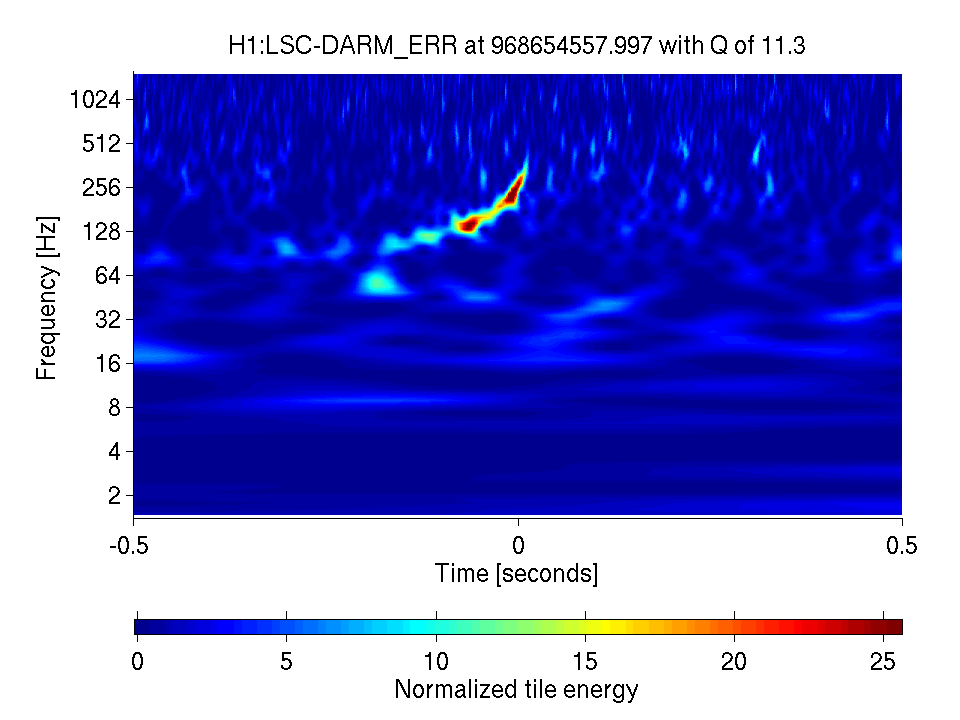
\includegraphics[width=0.5\linewidth]{figures/detchar/968654557_997314453_H1_LSC-DARM_ERR_1_00_spectrogram_whitened.png}
  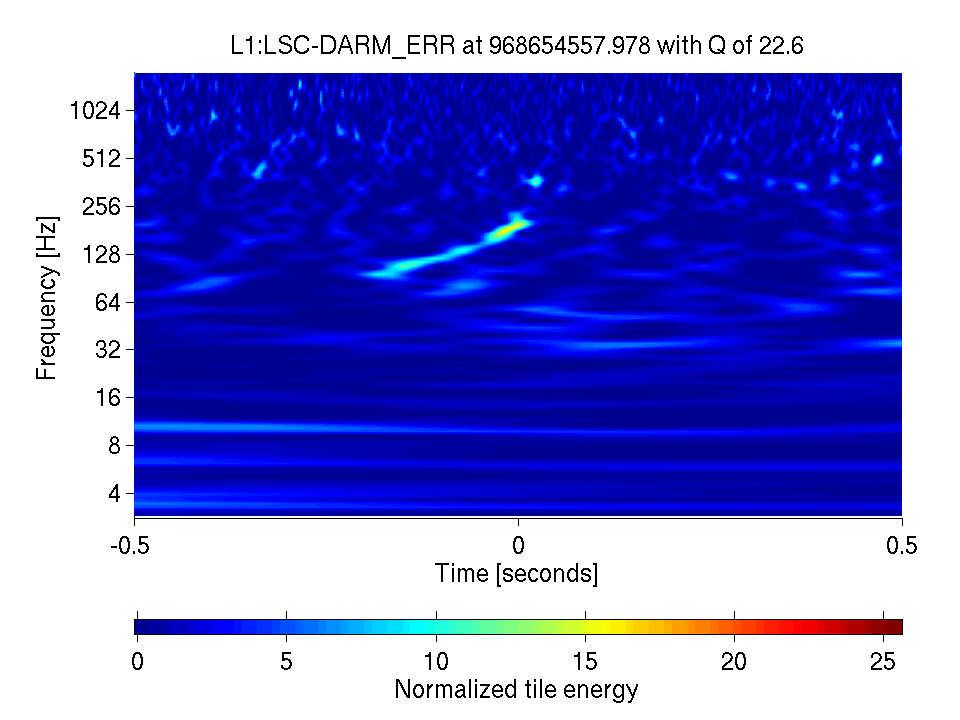
\includegraphics[width=0.5\linewidth]{figures/detchar/968654557_978027343_L1_LSC-DARM_ERR_1_00_spectrogram_whitened.png}
  \caption[Omega scans of the injection]{
  \label{f:daily_ihope_dog_omega}
H1 (left) and L1 (right) Omega scans of the injection as
generated by daily ihope.  Note the ``chirp'' shape which is the
expected pattern from a compact binary inspiral.}
\end{figure}%

\subsection{False Alarm Rate Estimate}

% https://www.lsc-group.phys.uwm.edu/ligovirgo/cbcnote/DailyDogHistograms

In order to determine the significance of this candidate event it was
necessary to compare it against the background.  The first such
comparison ranked the event against background triggers from the
two-week analysis in which it occurred as part of the standard ihope
pipeline.  However, the event had a larger combined new SNR value than
all background triggers, and hence had a false alarm probability of
zero.

In order to provide a more meaningful bound it was necessary to
increase the analysis time and/or number of slides to probe the
background more deeply. This is a complex and time-consuming process,
see (s6 paper) for details.  While this was underway we could begin to
bound the significance from daily ihope results.  This was done by
plotting histograms of all triggers throughout S6 and locating the
candidate triggers in the resulting distribution.  This analysis
differs from the full ihope pipeline in several respects.  However,
the goal was not a publishable result but only a rapid estimate.

To parallel the full analysis the results were broken into mass bins.
The low mass bin spans chirp masses up to $3.48\msun$, the medium mass
bin from $3.48-7.40 \msun$.  Likewise, category 1,2 and 3 vetoes were
applied to parallel the results of the full search.  30-millisecond
clustering was chosen to parallel the clustering used in the full
search.  There are several ways of reporting the new SNR of the
injection; the largest values reported by daily ihope, the largest
single-detector values reported by the full search, and the component
values of the largest combined new SNR reported by the full search.
All of these options are included on the plot.


The results are shown in figure \ref{f:daily_histogram_low} for the
low-mass bin and \ref{f:daily_histogram_medium} for the medium-mass
bin.  The result in both bins is qualitatively the same.  The
injection is close to the loudest event in H1 for all measures of new
SNR.  The injection does not stand out as far in L1, which was known
to be glitchier over the course of S6.


\begin{figure}
  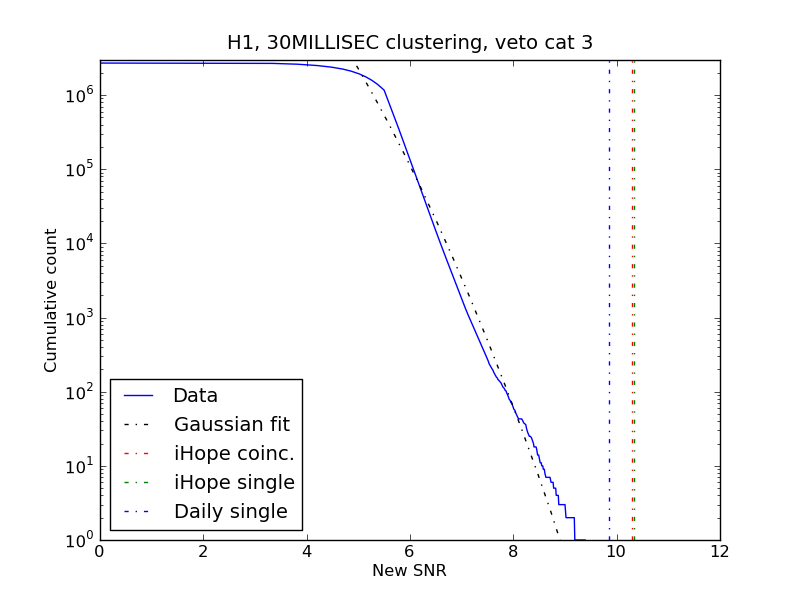
\includegraphics[width=0.5\linewidth]{figures/detchar/LM_H1_30MILLISEC_3_hist.png}
  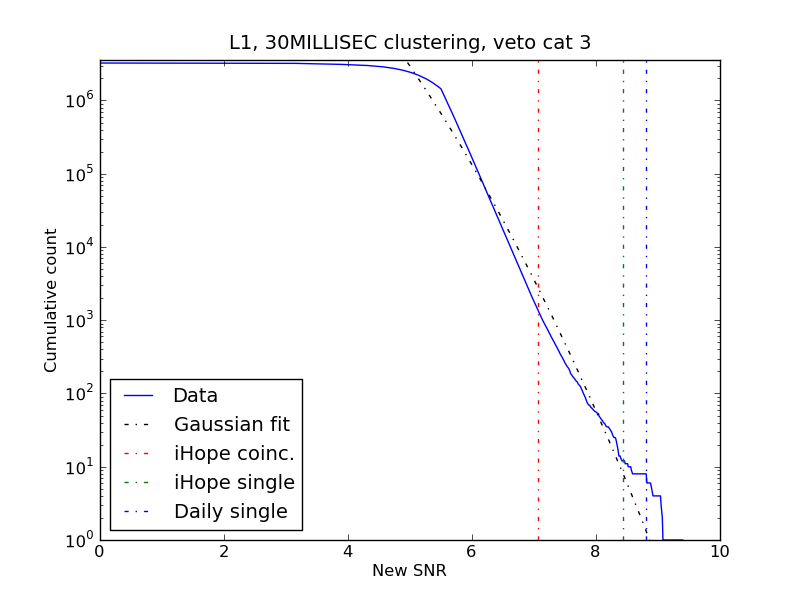
\includegraphics[width=0.5\linewidth]{figures/detchar/LM_L1_30MILLISEC_3_hist.png}
  \caption[Significance of the injection in the low-mass bin]{
  \label{f:daily_histogram_low}
Significance of the blind injection in the low-mass bin in 
H1 (left) and L1 (right).  Note the cumulative counts levels off
around between 5 and 5.5, indicating that there are few triggers with
smaller values.}
\end{figure}%



\begin{figure}
  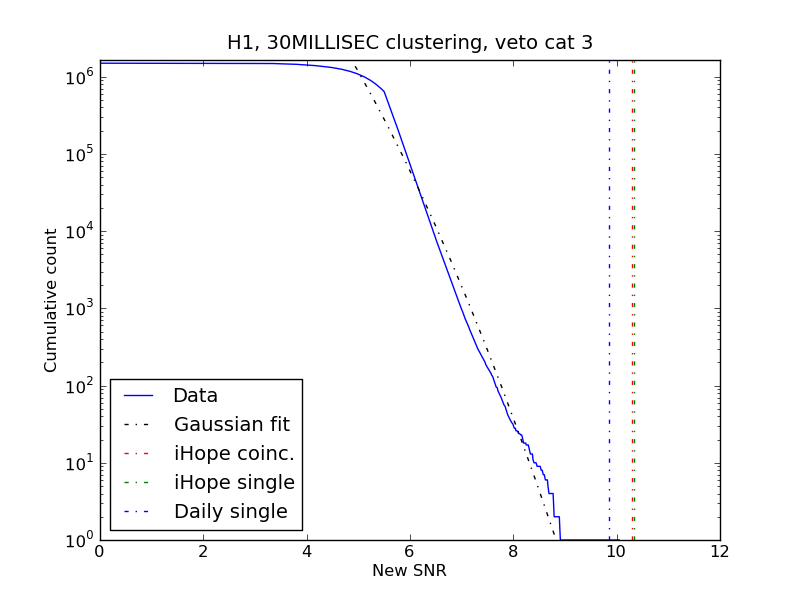
\includegraphics[width=0.5\linewidth]{figures/detchar/MM_H1_30MILLISEC_3_hist.png}
  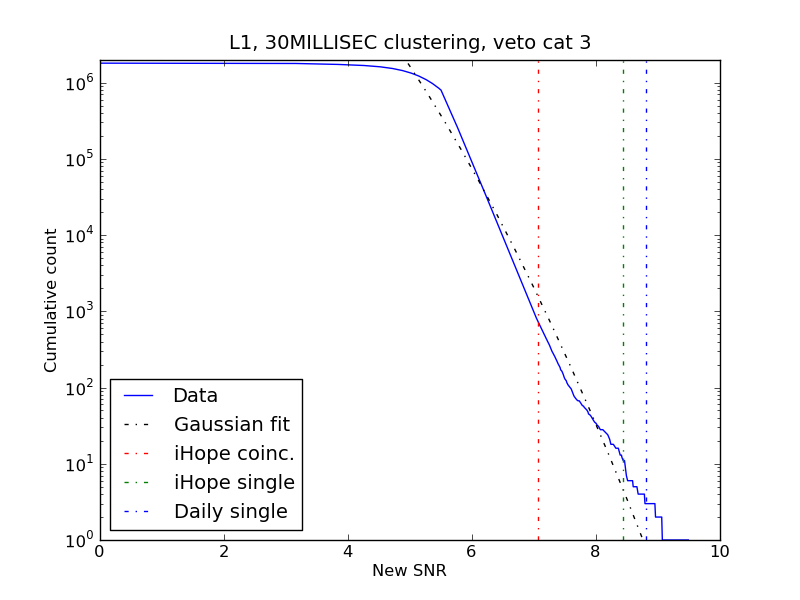
\includegraphics[width=0.5\linewidth]{figures/detchar/MM_L1_30MILLISEC_3_hist.png}
  \caption[Significance of the injection in the medium-mass bin]{
  \label{f:daily_histogram_medium}
Significance of the blind injection in the medium-mass bin in 
H1 (left) and L1 (right).  Note the cumulative counts levels off
around between 5 and 5.5, indicating that there are few triggers with
smaller values.}
\end{figure}%


From these results we can attempt to estimate a false alarm rate for
the injection as follows.   Model coincident triggers as a Bernoulli
trial where ``success'' is obtaining a coincidence with combined new
SNR greater than or equal to that of the injection.  Denote the
probability of success in a single trial as $P$.  Then the probability
of obtaining the first success after $k$ trials is a geometric
distribution, $Prob(k) = P(1-P)^{k-1}$, and the expected number of
trials before success is $1/P$.  Dividing this by the estimated number
of coincident triggers in a year gives the estimated number of years
required to obtain such a trigger by chance.

The rate of coincident triggers, $R$, in the full search was estimated
by choosing a few analysis chunks and dividing the number of H1L1
triggers by the analysis time, both of which are reported after the
coincidence step.  The average rate is approximately 0.004
coincidences per second of analysis time, or $N=126,144$ per year.
This is combined across all mass bins, the result will therefore be an
upper limit for any particular bin.

% CIT:
% /archive/home/sprivite/S6/lowmass/s6d_weeks33_34/968803143-970012887/full_data
% for i in `/bin/ls | grep H1L1-COIRE_FIRST_FULL_DATA `
% do
%  grep 'amount of time analysed' $i | cut -f7 -d' '
% done | awk '{s+=$1} END {print s}'
% 135254
%
% for i in `/bin/ls | grep H1L1-COIRE_FIRST_FULL_DATA `
% do
%  grep 'reconstructed' $i | cut -f7 -d' '
% done | awk '{s+=$1} END {print s}'
%
% 523
% so 523 / 135254 = 0.00387 coinc/sec
%
%
% LHO (dog)
% /archive/home/mtwest/CBC-s6d/weeks_31-32/lowmass_run/967593543-968803287/full_data
% Gives 
% 886 / 244515 = 0.00362 coinc/sec


We estimate $P$ by assuming a probability density function in each
detector of the form

\begin{equation}
P(\rho_\textrm{new}) = \left\{
  \begin{array}{lr}
    0  & \rho < 5.5 \\
    \exp\left(-\frac{\rho^2}{2\sigma^2}\right) & \rho_\textrm{new} \geq 5.5 \\
  \end{array} \right.
\end{equation}

The lower cutoff is approximate.  We do not threshold on new SNR, and
while we do threshold on$\rho > 5.5$ it is possible for $\chisq$ to
push the resulting new SNR down.  In addition, due to clustering, the
probability of obtaining low new SNR triggers is suppressed.  The fit
to the Gaussian portion of the curves is show on  figures
\ref{f:daily_histogram_low} and \ref{f:daily_histogram_medium}, and
the obtained values are shown in table \ref{tab:daily_ihope_sigmas}.

\begin{table*}
\begin{center}
\begin{tabular}{l | l l}
   & $\sigma_H$ & $\sigma_L$ \\
\hline
Low mass bin    & 0.98 & 0.96 \\
Medium mass bin & 0.99 & 0.97 \\
\end{tabular}
\end{center}
  \caption[Fit values for SNR histograms]{
  \label{tab:daily_ihope_sigmas}
$\sigma$ values obtained by fitting Gaussians to daily
ihope trigger counts.}
\end{table*}

The joint PDF is then

\begin{equation}
P(\rho_H,\rho_L) = \frac{1}{A}
\int_{\rho_L = 5.5}^{\sqrt{\rho_i^2 - \rho_L^2}}
\int_{\rho_H = 5.5}^{\sqrt{\rho_i^2 - 5.5^2}}
\exp\left(-\frac{\rho_H^2}{2\sigma^2}\right)
\exp\left(-\frac{\rho_L^2}{2\sigma^2}\right)
\,d\rho_H
\,d\rho_L
\end{equation}

where $A$ is the normalization obtained by taking the upper limits of
both integrals to infinity.  This may be simplified by means of the
substitutions

\begin{align*}
s      &= \frac{\rho_H}{\sqrt{2}\sigma_H} \\
s_{\mathrm{low}}  &= \frac{5.5}{\sqrt{2}\sigma_H} \\
s_{\mathrm{high}} &= \frac{sqrt{\rho_i^2 - 5.5^2}}{\sqrt{2}\sigma_H} \\
t      &= \frac{\rho_L}{\sqrt{2}\sigma_L} \\
t_{\mathrm{low}}  &= \frac{5.5}{\sqrt{2}\sigma_L} \\
t_{\mathrm{high}}(s) &= \frac{\sqrt{\rho_i^2 - 2 \sigma_H^2 s^2}}{\sqrt{2}\sigma_L} \\
\end{align*}

in terms of which the normalization is

\begin{equation}
A = \frac{\pi}{2} \sigma_x \sigma_y \left[
1 - \erf(s_{\mathrm{low}}) - \erf(t_{\mathrm{low}}) + \erf(s_{\mathrm{low}})\erf(t_{\mathrm{low}})
\right]
\end{equation}

where $\erf$ is the error function.  The probability of obtaining a
trigger with combined new SNR larger then the injection is then

\begin{align*}
P &= 1 - \frac{\pi\sigma_L \sigma_H}{2 A} \bigg[
\frac{2}{\pi} \int_{s_{\mathrm{low}}}^{s_{\mathrm{high}}} e^{-s^2}
\erf(t_{\mathrm{high}}(s))\,ds \nonumber \\
&\quad - \erf(t_{\mathrm{low}}) \erf(s_{\mathrm{high}})  
+ \erf(s_{\mathrm{low}}) \erf (t_{\mathrm{low}}) \bigg] \\
\end{align*}


\iffalse
\begin{equation}
P(\rho_H,\rho_L) = 
\frac{4}{2\pi \sigma_H \sigma_L} 
\exp\left(
-\frac{\rho_H^2}{2\sigma_H^2} -\frac{\rho_L^2}{2\sigma_L^2}
\right)
\end{equation}

where the factor $4$ comes from considering only the quadrant where
both SNRs are positive.

The probability of obtaining a trigger with new SNR greater than
that of the injection, $\rho_i$, is then

\begin{align}
P = 
\frac{4}{2\pi \sigma_H \sigma_L} 
\int_{\rho_H^2 + \rho_L^2 > \rho_i^2}
\exp\left(
-\frac{\rho_H^2}{2\sigma_H^2} -\frac{\rho_L^2}{2\sigma_L^2}
\right)
\,d\rho_H\,d\rho_L
\end{equation}

Introducing a temporary variable $M = \rho_L \sigma_H/\sigma_L$, going to polar
coordinates, evaluating the integral over $r$ and simplifying gives


\begin{equation}
P(\rho_c^2 > \rho_i^2|\textrm{coincidence}) = 
\frac{1}{2\pi \sigma_H \sigma_L} 
\frac{\sigma_L}{\sigma_H}
\int_{\rho_H^2 + (\sigma_L/\sigma_H)^2 M^2 \leq \rho_i^2}
\exp\left(
-\frac{\rho_H^2}{2\sigma_H^2} -\frac{M^2}{2\sigma_H^2}
\right)
\,d\rho_H\,dM
\end{equation}



\begin{equation}
P = 
\frac{1}{2\pi \sigma_H \sigma_L} 
\frac{\sigma_L}{\sigma_H}
\int_{r^2\cos^2\theta + (\sigma_L/\sigma_H)^2 r^2\sin^2\theta \leq \rho_i^2}
\exp\left(
-\frac{r^2\cos^2\theta}{2\sigma_H^2} -\frac{r^2\sin^2\theta}{2\sigma_H^2}
\right)
r\, dr\, d\theta
\end{equation}


\begin{equation}
P = 
\frac{1}{2\pi \sigma_H \sigma_L} 
\frac{\sigma_L}{\sigma_H}
\int_{r^2\cos^2\theta + (\sigma_L/\sigma_H)^2 r^2\sin^2\theta \leq \rho_i^2}
\exp\left( -\frac{r^2}{2\sigma_H^2} \right)
r\, dr\, d\theta
\end{equation}


\begin{equation}
P = 
\frac{1}{2\pi \sigma_H \sigma_L} 
\frac{\sigma_L}{\sigma_H}
\sigma_H^2
\int_0^{2\pi}
\left( 1 - 
\exp\left(
  -\frac{1}{2\sigma_H^2} 
   \frac{\rho_i^2}
        {\cos^2\theta + (\sigma_L/\sigma_H)^2 \sin^2\theta} 
\right)
\right)
d\theta
\end{equation}

\begin{equation}
P = \frac{4}{2\pi}
\int_0^{\pi/2}
\exp\left(
  -\frac{1}{2} 
   \frac{\rho_i^2}
        {\sigma_H^2 \cos^2\theta + \sigma_L^2 \sin^2\theta} 
\right)
d\theta
\end{equation}

\fi

This integral can be evaluated numerically.  Henceforth we focus on
the medium mass bin, as that was the bin with the most significant
trigger with a combined new SNR $\rho_i = 12.5$.  The result is
$P = 1.4 \times 10^{-20}$, which gives a false alarm rate of
1 event in 

\begin{equation}
\frac{1.0}{1.4 \times 10^{-26}} \times \frac{1}{126,144}
= 8.6\times 10^{24}\quad\textrm{years}
\end{equation}

This grossly underestimates the FAR calculated using time slides based
on the full analysis, which gives 1 in 7,000 years.  There is no
simple factor that explains this discrepancy; the two analyses are
significantly different, and in particular the real search uses a
two-stage pipeline that makes it difficult to reason about the results
based on the output of single-stage single-ifo triggers.  However,
this does suggest an alternative method to estimate FARs for a
single-stage pipeline which is currently in development.

\subsection{Front-end code verification}

% http://www.gravity.phy.syr.edu/dokuwiki/doku.php?id=larne:frontendcode
% https://dcc.ligo.org/cgi-bin/private/DocDB/ShowDocument?docid=39122
% https://dcc.ligo.org/cgi-bin/private/DocDB/ListBy?authorid=272

Before the collaboration could claim a detection it was necessary to
perform extensive checks to remove, or at least reduce, the
possibility that the trigger was due to any source other than a
gravitational wave.  Consequently many components of the
interferometer were subject to scrutiny.  One such component was the
\emph{front-end control code}, which is responsible for \checkme{FILL
IN DETAILS}.  This code is updated occasionally as new systems are
added or bugs are found and fixed.   To verify that the most recent
change preceding the event did not significantly change the behavior
of the instruments we compared histograms of triggers from daily ihope
before and after these changes.

Two weeks prior to and following the most recent code changes at each
site were selected.  SNR histograms are shown in figure \ref{f:code_changes}.
There is a slight variation in H1, somewhat larger in L1.  More
rigorous testing could have been done, one possibility would be to
determine rates from several two-week periods before the code change
in order to estimate the standard deviation in each SNR bin, and then
checking whether the rates after the change fall within one sigma.
However, the detection committee did not feel this level of analysis
was necessary, and based on the plots in figure \ref{f:code_changes}
concluded:


\begin{figure}
  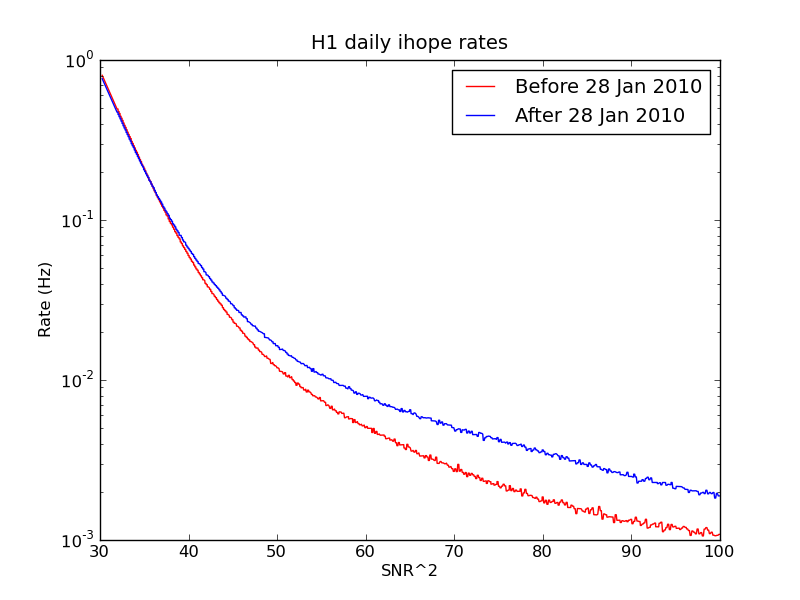
\includegraphics[width=0.5\linewidth]{figures/detchar/frontendtest_h1_log_2.png}
  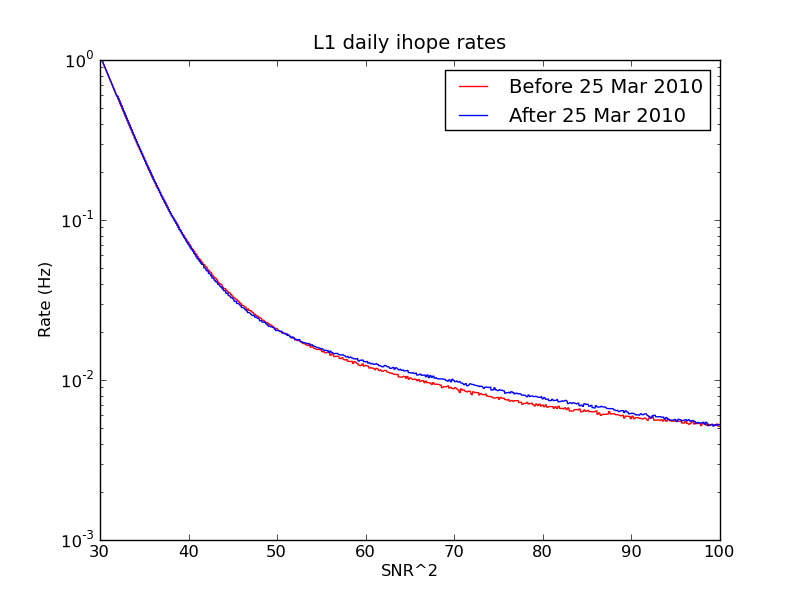
\includegraphics[width=0.5\linewidth]{figures/detchar/frontendtest_l1_log_2.png}
  \caption[SNR histograms before and after code changes.] {
  \label{f:code_changes}
SNR histograms comparing periods before and after 
front-end code changes at H1 (left) and L1 (right).}
\end{figure}%


\begin{quote}
  Thus, to the extent allowed by the methods we adopted, there is no
  evidence for any malfunction in the front-end code of the
  interferometers. (cite https://dcc.ligo.org/cgi-bin/private/DocDB/ShowDocument?docid=39122)
\end{quote}

\subsection{Loud-SNR veto}


% tot_time, tot_count
% veto_time, veto_count

% $ ./check_flags.py L1
% 798720 2890507
%    880   12578
% $ ./check_flags.py H1
% 647168 1692904
%    416    6452


